
\documentclass[a4paper,oneside,anyway]{book}%[a4paper,titlepage,oneside]{book}

%\usepackage{amsthm,amssymb,amsmath,mathtools}
\usepackage[font=small,labelfont=bf]{caption}

\usepackage[titles]{tocloft}
%\usepackage{minitoc}
\usepackage{float}
\usepackage{fancyhdr}
\usepackage[headheight=110pt]{geometry}
 \geometry{
 a4paper,
 %total={210mm,297mm},
 left=25mm,
 right=40mm,
 top=30mm,
 bottom=30mm,
 }
\usepackage{titlesec}
\usepackage{longtable}
\usepackage{titlepic}
\usepackage[nottoc,notlot,notlof]{tocbibind}
\usepackage{algorithm}
\usepackage{algorithmic}
%\definecolor{MSBlue}{rgb}{.204,.353,.741}
\usepackage{hyperref}
\hypersetup{
   % bookmarks=true,         % show bookmarks bar?
    unicode=true,          % non-Latin characters in Acrobat’s bookmarks
    pdftoolbar=true,        % show Acrobat’s toolbar?
    pdfmenubar=true,        % show Acrobat’s menu?
    pdffitwindow=false,     % window fit to page when opened
    pdfstartview={FitH},    % fits the width of the page to the window
    pdftitle={Information Diffusion report},    % title
    pdfauthor={Hassan Abedi},     % author
    pdfsubject={Information Diffusion},   % subject of the document
    pdfcreator={hassan abedi},   % creator of the document
    pdfproducer={hassan abedi}, % producer of the document
    pdfkeywords={Information Diffusion} {Social Networks}, % list of keywords
    pdfnewwindow=true,      % links in new window
    colorlinks=true,       % false: boxed links; true: colored links
    linkcolor=black,%blue,%MSBlue,          % color of internal links (change box color with linkbordercolor)
    citecolor=black,        % color of links to bibliography
    filecolor=magenta,      % color of file links
    urlcolor=black %cyan    % color of external links
    }

\usepackage{hyperref}
\usepackage{xepersian}
\usepackage[nospace,noadjust]{cite}
\usepackage{enumitem}
\usepackage{zref-perpage}
\usepackage{textcomp}
\usepackage{graphicx}
\usepackage{subcaption}
\usepackage{url}
\usepackage{footmisc}
\usepackage[utf8]{inputenc}
\usepackage{setspace}
\renewcommand{\baselinestretch}{2} 
\usepackage{lastpage}
\renewcommand{\citeleft}{[}
\renewcommand{\citeright}{]}
\usepackage{breakcites}
\usepackage{setspace}

\newlength\mylenprt
\newlength\mylenchp
\newlength\mylenapp

\renewcommand\cftpartpresnum{~}
\renewcommand\cftchappresnum{\chaptername~}
\renewcommand\cftchapaftersnum{:}

\settowidth\mylenprt{\cftpartfont\cftpartpresnum\cftpartaftersnum}
\settowidth\mylenchp{\cftchapfont\cftchappresnum\cftchapaftersnum}
\settowidth\mylenapp{\cftchapfont\appendixname~\cftchapaftersnum}
\addtolength\mylenprt{\cftpartnumwidth}
\addtolength\mylenchp{\cftchapnumwidth}
\addtolength\mylenapp{\cftchapnumwidth}

\setlength\cftpartnumwidth{\mylenprt}
\setlength\cftchapnumwidth{\mylenchp}	

\makeatletter
{\def\thebibliography#1{\chapter*{\refname\@mkboth
   {\uppercase{\refname}}{\uppercase{\refname}}}\list
   {[\arabic{enumi}]}{\settowidth\labelwidth{[#1]}
   \rightmargin\labelwidth
   \advance\rightmargin\labelsep
   \advance\rightmargin\bibindent
   \itemindent -\bibindent
   \listparindent \itemindent
   \parsep \z@
   \usecounter{enumi}}
   \def\newblock{}
   \sloppy
   \sfcode`\.=1000\relax}}
\makeatother

\renewcommand{\bibname}{مراجع}
\newcommand{\head}[1]{\textnormal{\textbf{#1}}}
\newtheorem{thm}{Theorem}[chapter]
\newtheorem{lem}[thm]{Lemma}
\theoremstyle{definition}
\newtheorem{dfn}[thm]{Definition}

\usepackage{fontspec}
\settextfont[Scale=1.4]{B Nazanin}
\setdigitfont[Scale=1]{B Nazanin}
\setlatintextfont[Scale=1]{Times New Roman}
\defpersianfont\titlefont[Scale=1]{B Nazanin}


\makeatletter
\def\tagform@#1{\maketag@@@{)#1(\@@italiccorr}}
\makeatother

\numberwithin{table}{section}
\numberwithin{equation}{section}
\numberwithin{figure}{section}

\makeatletter
     \renewcommand*\l@figure{\@dottedtocline{1}{1em}{3.2em}}
\makeatother

\makeatletter
     \renewcommand*\l@table{\@dottedtocline{1}{1em}{3.2em}}
\makeatother

\newcommand\persiangloss[2]{#1\dotfill\lr{#2}\\}
% دستوری برای تعریف واژه‌نامه فارسی به انگلیسی 
\newcommand\englishgloss[2]{#2\dotfill\lr{#1}\\} %{اگه می خواین نسخه‌ی چاپی درست کنید}
\usepackage{amsthm,amssymb,amsmath,mathtools}
\usepackage[font=small,labelfont=bf]{caption}

\usepackage[titles]{tocloft}
%\usepackage{minitoc}
\usepackage{float}
\usepackage{fancyhdr}
\usepackage[headheight=110pt]{geometry}
 \geometry{
 a4paper,
 %total={210mm,297mm},
 left=25mm,
 right=40mm,
 top=30mm,
 bottom=30mm,
 }
\usepackage{titlesec}
\usepackage{longtable}
\usepackage{titlepic}
\usepackage[nottoc,notlot,notlof]{tocbibind}
\usepackage{algorithm}
\usepackage{algorithmic}
%\definecolor{MSBlue}{rgb}{.204,.353,.741}
\usepackage{hyperref}
\hypersetup{
   % bookmarks=true,         % show bookmarks bar?
    unicode=true,          % non-Latin characters in Acrobat’s bookmarks
    pdftoolbar=true,        % show Acrobat’s toolbar?
    pdfmenubar=true,        % show Acrobat’s menu?
    pdffitwindow=false,     % window fit to page when opened
    pdfstartview={FitH},    % fits the width of the page to the window
    pdftitle={Information Diffusion report},    % title
    pdfauthor={Hassan Abedi},     % author
    pdfsubject={Information Diffusion},   % subject of the document
    pdfcreator={hassan abedi},   % creator of the document
    pdfproducer={hassan abedi}, % producer of the document
    pdfkeywords={Information Diffusion} {Social Networks}, % list of keywords
    pdfnewwindow=true,      % links in new window
    colorlinks=false,       % false: boxed links; true: colored links
    linkcolor=blue,%blue,%MSBlue,          % color of internal links (change box color with linkbordercolor)
    citecolor=blue,        % color of links to bibliography
    filecolor=magenta,      % color of file links
    urlcolor=magneta %cyan    % color of external links
    }

\usepackage{hyperref}
\usepackage{xepersian}
\usepackage[nospace,noadjust]{cite}
\usepackage{enumitem}
\usepackage{zref-perpage}
\usepackage{textcomp}
\usepackage{graphicx}
\usepackage{subcaption}
\usepackage{url}
\usepackage{footmisc}
\usepackage[utf8]{inputenc}
\usepackage{setspace}
\renewcommand{\baselinestretch}{2} 
\usepackage{lastpage}
\renewcommand{\citeleft}{[}
\renewcommand{\citeright}{]}
\usepackage{breakcites}
\usepackage{setspace}

\newlength\mylenprt
\newlength\mylenchp
\newlength\mylenapp

\renewcommand\cftpartpresnum{~}
\renewcommand\cftchappresnum{\chaptername~}
\renewcommand\cftchapaftersnum{:}

\settowidth\mylenprt{\cftpartfont\cftpartpresnum\cftpartaftersnum}
\settowidth\mylenchp{\cftchapfont\cftchappresnum\cftchapaftersnum}
\settowidth\mylenapp{\cftchapfont\appendixname~\cftchapaftersnum}
\addtolength\mylenprt{\cftpartnumwidth}
\addtolength\mylenchp{\cftchapnumwidth}
\addtolength\mylenapp{\cftchapnumwidth}

\setlength\cftpartnumwidth{\mylenprt}
\setlength\cftchapnumwidth{\mylenchp}	

\makeatletter
{\def\thebibliography#1{\chapter*{\refname\@mkboth
   {\uppercase{\refname}}{\uppercase{\refname}}}\list
   {[\arabic{enumi}]}{\settowidth\labelwidth{[#1]}
   \rightmargin\labelwidth
   \advance\rightmargin\labelsep
   \advance\rightmargin\bibindent
   \itemindent -\bibindent
   \listparindent \itemindent
   \parsep \z@
   \usecounter{enumi}}
   \def\newblock{}
   \sloppy
   \sfcode`\.=1000\relax}}
\makeatother

\renewcommand{\bibname}{مراجع}
\newcommand{\head}[1]{\textnormal{\textbf{#1}}}
\newtheorem{thm}{Theorem}[chapter]
\newtheorem{lem}[thm]{Lemma}
\theoremstyle{definition}
\newtheorem{dfn}[thm]{Definition}

\usepackage{fontspec}
\settextfont[Scale=1.4]{B Nazanin}
\setdigitfont[Scale=1]{B Nazanin}
\setlatintextfont[Scale=1]{Times New Roman}
\defpersianfont\titlefont[Scale=1]{B Nazanin}


\makeatletter
\def\tagform@#1{\maketag@@@{)#1(\@@italiccorr}}
\makeatother

\numberwithin{table}{section}
\numberwithin{equation}{section}
\numberwithin{figure}{section}

\makeatletter
     \renewcommand*\l@figure{\@dottedtocline{1}{1em}{3.2em}}
\makeatother

\makeatletter
     \renewcommand*\l@table{\@dottedtocline{1}{1em}{3.2em}}
\makeatother

\newcommand\persiangloss[2]{#1\dotfill\lr{#2}\\}
% دستوری برای تعریف واژه‌نامه فارسی به انگلیسی 
\newcommand\englishgloss[2]{#2\dotfill\lr{#1}\\}

\begin{document}
\pagestyle{empty}

\pagenumbering{harfi} % alphateical 
\tableofcontents \newpage
\listoffigures \newpage
\listoftables \newpage
\pagestyle{fancy}
\lhead{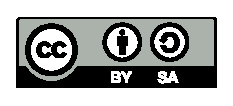
\includegraphics[width=2.1cm]{figures/by-sa}}
\DefaultMathsDigits

\usepackage{titlesec}
\titlespacing\section{0pt}{12pt plus 4pt minus 2pt}{5pt plus 5pt minus 2pt}
\titlespacing\subsection{0pt}{12pt plus 4pt minus 2pt}{5pt plus 5pt minus 2pt}
\titlespacing\subsubsection{0pt}{12pt plus 4pt minus 2pt}{5pt plus 5pt minus 2pt}

\pagenumbering{arabic} % numerical

\chapter{مقدمه} 
\newpage


\section{کلیات}
\noindent {
شبکه‌های اجتماعی جزو جدا نشدنی زندگی جامعه انسانی می باشند. در گذشته این شبکه‌ها با محدودیت‌های زیادی جهت مطالعه روبرو بوده اند. با گسترش روزافزون شبکه‌های اجتماعی آنلاین در ده سال گذشته بسیاری از محدودیتهای ارتباطی ناشی از فواصل زیاد جغرافیایی اعضا ازبین رفته است، که باعث بزرگ شدن اندازه ی شبکه‌های اجتماعی مورد بحث شده است \cite{musial_social_2013}. همین طور تکنولوژی لازم برای ذخیره و بازیابی و واکاویی اطلاعات مربوط به این شبکه‌های عظیم و کاربرانشان در دسترس می‌باشد.
\\
\indent
نمود شبکه‌های اجتماعی مورد بحث سایت‌هایی مانند فیسبوک و گوگل‌پلاس و اورکوت می‌باشند. این سایت‌هابه کاربران خود سرویس هایی ارایه می دهند که به کمک این سرویس ها اعضا قادر به اشتراک گذاری محتوای اجتماعی خودشان با دیگران می‌باشند. 
محتوای این افراد در ظرف هایی مانند متن و تصویر و ویدیو در سطح این شبکه‌ها پخش می شود. این امر از این جهت برای محققان مورد علاقه است که محتوای اجتماعی در جریان در این سایت‌ها قدرت تاثیرگذاری روی رفتار و منش اعضای این شبکه‌ها را به سادگی داراست. از طرف دیگر محتوای مورد توجه یک کاربر می‌تواند علایق و تمایلات وی به خوبی نشان دهد، از این رو تحقیق و پژوهش در امر چگونگی فرایند پخش محتوای اطلاعاتی در سطح شبکه های اجتماعی آنلاین مورد توجه محققانی از رشته‌های ‌مختلف مانند جامه‌شناسی و اقتصاد و کامپیوتر بوده است.
\\
\indent
اولین کارهای مربوط به امر پخش اطلاعات به اوایل قرن بیستم در باره‌‌ی چگونگی روند بکارگیری فناوری های نوین بوده است \cite{rogers2010diffusion}. برای نمونه به چگونگی پخش امر استفاده‌ی کشاورزان از دانه‌های اصلاح شده‌ی محصولات به جای دانه‌های مرسوم در چند ایالت آمریکا در دهه‌ی ۳۰ قرن گذشته.


}

\section{هدف سمینار}

در این سمینار به بررسی اجزای مهم تشکیل دهنده‌ی فرایند پخش اطلاعات می پردازیم. هم‌چنین مدل‌های ارایه شده برای مدل‌سازی و تحلیل این فرایند را مورد بررسی قرار خواهیم داد. البته پخش اطلاعات را می‌توان از زوایای مختلفی مورد مطالعه و تحقیق قرار داد، مانند طراحی و ساخت مدل‌های توصیفی از فرایند پخش اطلاعات، بررسی موضوعات متنی مورد توجه\cite{guille_information_2013}، یافتن افراد تاثیرگذار \cite{cha_measuring_2010} و پیش‌بینی انتشار\cite{cheng_can_2014} که در این نوشته بیشتر به بعد مدل‌سازی این فرایند پرداخته شده است.
\section{ساختار این گزارش}
\begin{persian}
\noindent
فصل دوم این نوشته به آشنایی با مفاهیم و مطالب مرتبط پیرامون پخش شدن اطلاعات در سطح شبکه‌های اجتماعی آنلاین می‌پردازد تا خواننده را با کلیت موضوع مورد‌ بحث و موارد مطرح در زمینه‌ی پژوهش ‌و تجزیه‌ و تحلیل فرایند‌ عنوان این نوشته به طور عام آشناتر کند، هم‌چنین به معرفی چند جز تاثیرگذار امر پخش‌ اطلاعات در سطح شبکه‌های اجتماعی آنلاین خواهیم پرداخت. لذا در صورت آشنایی با موارد مطرح در این فصل خواننده می‌تواند از این مطالب بگذرد و به فصل دوم برای ادامه‌ی مطالعه مراجعه کند.
\\
\indent 
در فصل سوم نیز به معرفی و مقایسه‌ی مدل‌های مطرح ‌شده برای مدل‌سازی چگونگی فرایند پخش و همه‌گیری\پانویس{\lr{ Epidemic}} و شایعه به طور عام و طور خاص‌تر کاربری این مدل‌ها در مدل‌سازی فرایند پخش اطلاعات در سطح شبکه‌های اجتماعی آنلاین اختصاص داده شده است. فصل چهار هم به جمع‌بندی و نتیجه‌گیری مطالب گفته‌شده در فصول پیشین خواهد پرداخت.
 
\end{persian}




\chapter{مفاهیم مربوط به شبکه‌‌های اجتماعی و اجزای فرایند پخش اطلاعات}
%\minitoc
\newpage

\section{مقدمه}
\noindent {
در این فصل در ابتدا به معرفی شبکه‌های اجتماعی آنلاین و مفاهیم مرتبط پیرامون آن‌ها مانند هوموفیلی و فرضیه قدرت اتصال‌ها و همین‌طور شرح نمود گرافی این شبکه‌ها می پردازیم. در ادامه تعریفی از فرایند پخش اطلاعات به موضوع یکی از فرایند‌های مهم در جریان شبکه‌های اجتماعی آنلاین ارایه می دهیم. به همراه مابقی تعاریف مرتبط مانند میم و اقتصاد توجه، در انتها به جمع‌بندی آنچه گفته شد می‌پردازیم. 

}

%\newpage
\section{شبکه‌‌های اجتماعی آنلاین}
\begin{persian}
\noindent
یک شبکه‌ی اجتماعی متشکل از مجموعه‌ای از افراد می‌باشد که با‌هم به گونه‌ای رابطه دارند \cite{easley_networks_2010}. وجود شبکه‌های اجتماعی پدیده‌ای نوع و تازه نمی‌باشد، ولی ظهور اینترنت و در پی آن برپا‌شدن سایت‌‌‌هایی مثل توییتر و فیسبوک که چندصد میلیون کاربر فعال در لحظه را به‌هم متصل می‌کنند سبب از بین رفتن خیلی از محدودیت‌های مکانی و جغرافیایی‌ گذشته برای تشکیل اجتماعات مجازی آنلاین شده است. مثلا فیسبوک در طول‌یک ماه به طور متوسط در حدود ۱ میلیارد\زیرنویس{ فیسبوک به کاربری که در ۳۰ روز گذشته به حساب خود وارد شده باشد و با دیگر اعضا به تعامل پرداخته باشد کاربر فعال می‌گوید.} \cite{taxidou_realtime_2013} کاربر فعال دارد، کاربران توییتر هم که از مرز چند صد میلیون گذشته اند روزانه حدود ۴۰۰ میلیون توییت ارسال می‌کنند. به طور دقیق‌تر این دو سایت و دیگر وبسایت‌های اجتماعی آنلاین سرویس‌هایی شامل دراختیار قراردادن صفحه‌ای اختصاصی برای پیام‌‌ها و محتوای تولیدشده توسط کاربر ارایه می دهند. این امر امکان ارتباط کاربر با کاربران دیگر و پیگیری و به‌اشتراک‌قراردادن محتوا با دیگران را فراهم می سازد 
\cite{guille_information_2013}.
\\\indent
از لحاظ بزرگی ابعاد داده‌ی تولیدی کاربران این سایت‌ها، چگونگی استخراج دانش و اطلاعات‌ کاربران یکی از بحث‌های داغ روز در حوزه‌ی ابر داده\پانویس { Big Data} می‌باشد. برای مثال می‌قدرت ادعا کرد که داده‌ی تولیدی از توییت‌های\footnote{ توییت به پیام‌هایی اطلاق می‌شود که کاربران توییتر می‌قدرتند تولید و ارسال کنند. این پیام ‌‌ها از کم تر از ۱۴۱ حرف تشکیل می‌شوند و می‌قدرتند به همراه هشتگ(رشته‌ای از حروف که با \lr{\#} شروع شود.) و‌یا فایل تصویری و‌یا فیلم و پیوند ارسال شوند.} کاربران توییتر پیچیده‌ترین نوع داده‌ی تولید‌شده در سطح وب می‌باشد \cite{krishnan_data_2013}.
به طور کلی‌ یکی از موارد مطرح امروزی پیرامون این سایت‌ها چگونگی استفاده از این دریای اطلاعات برای حل مشکلاتی می‌باشد که تا چندی‌پیش حلشان غیر ممکن می‌نمود.
 \begin{figure}[H]
 \centering
 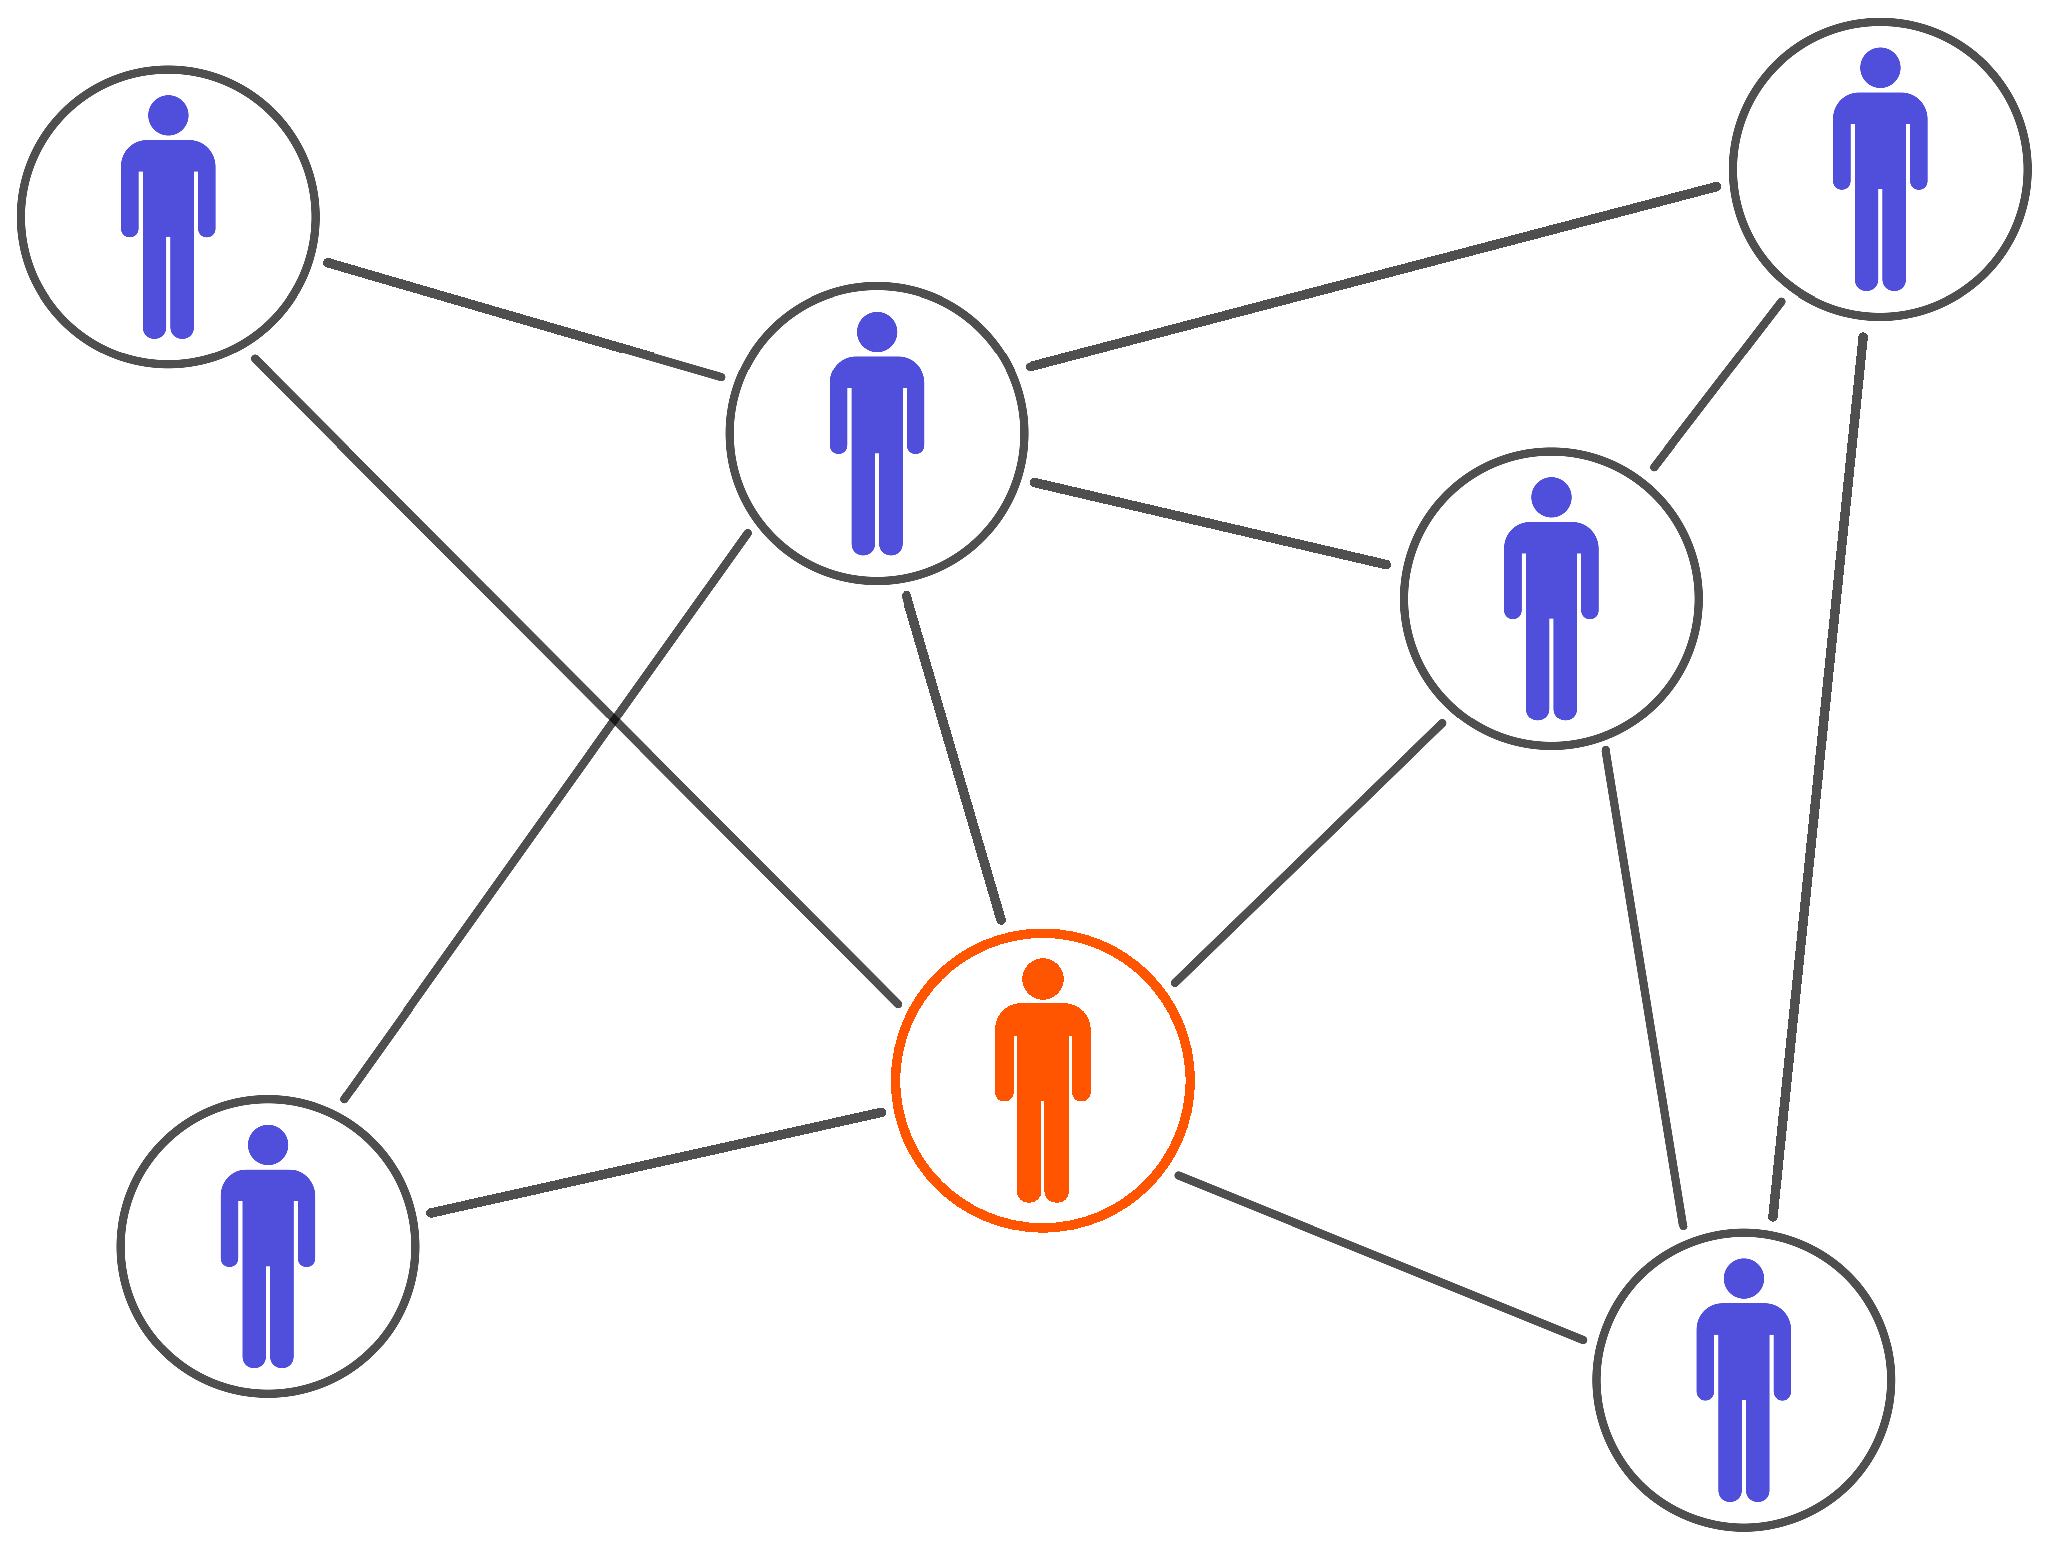
\includegraphics[scale=0.25]{figures/sn1}
 \caption[شبکه‌ی اجتماعی]
 {نمایی کلی از ‌یک شبکه‌ی اجتماعی.}
\end{figure}
\indent
\end{persian}
%\newpage
\subsection{نظریه گراف ‌‌ها}
\begin {persian}
 \noindent
 نظریه‌ی گراف‌ها علاوه بر کاربرد‌‌های فراوانی که در بسیاری از زمینه‌های علمی‌ و مهندسی دارد برای نشان‌دادن و مدل‌سازی ساختار شبکه‌های اجتماعی نیز بکار برده می‌شود.‌ یک شبکه‌ی اجتماعی‌ یک گراف پویاست \cite{easley_networks_2010} که رشد و نمو آن و همین‌طور تشکیل پیوندهای جدید در آن تابعی از زمان است. البته در اکثر اوقات از‌ یک تصویر لحظه‌ای \cite{guille_information_2013} ایستا که ساختار شبکه‌ی اجتماعی مورد نظر را در لحظه‌ی خاصی نشان می‌دهد برای توصیف آن شبکه‌‌‌ اجتماعی استفاده می‌شود. گراف مورد بحث $G=(V,E)$ به صورت مجموعه‌ای از رأس ‌‌ها(گره‌ها) با نام $V$ و مجموعه‌ای از‌ یال‌ها(پیوندها) به‌نام $E=\{ e_{ab}| a,b \in V\}$ نشان داده می‌شود. گراف حاصل می‌تواند جهت‌دار و‌یا بی جهت باشد برای مثال می‌قدرت در توییتر ارتباط‌هایی که دو طرفه می‌باشند، ‌یعنی هر دو طرف توییت‌‌ها و پیام‌های دیگری را دنبال می‌کند به صورت بی جهت در نظر گرفت و ارتباطاتی را که فقط‌ یک طرف دریافت کننده‌ی توییت‌هاست به صورت جهت‌دار نشان داد. همچنین گراف حاصل می‌تواند وزن دار باشد بدین معنا که به هر عضو مجموعه‌ی $E$ عددی را به موضوع وزن به نام $w_
e$ نسبت 
داد. \\
 \indent 
گراف‌های مورد بحث در زمینه شبکه‌‌‌های اجتماعی 
دارای خواص مشترک جالبی مثل کمی‌ فاصله هندسی\پانویس { Geodic distance } بین گره‌ها هستند، \cite{watts_six_2004, boccaletti_complex_2006} که نشان دهنده‌ی پدیده‌ی \lr{Small-world} می‌باشد. هم چنین تعداد‌ یال ‌‌های‌ یک گره تابعی از توزیع‌‌‌های \lr{Heavy-tailed} می‌باشد \cite{boccaletti_complex_2006}.
در جدول صفحه بعد خصوصیت‌های مطرح گراف حاصل از شبکه‌های اجتماعی را مشاهده می‌نمایید.
\\
\begin{table}[H]
%\label{tab:SNGModels}
\centering {
\onehalfspacing
 {\small
 \begin{tabular}{ | l | l | p{4.3cm} |}
 \hline
 {خصوصیت گراف شبکه‌ی اجتماعی} & {رابطه } & {توضیحات} \\ 
 \hline
 
 \lr{power law degree distribution} & $P(x) \sim x^{-\alpha}$ & $P(x)$
 احتمال این را که گره‌ای از $G$ دارای $x$‌یال باشد نشان می‌دهد. ضمنا $\alpha$ عدد ثابتی است که با آزمایش محاسبه می‌شود. \\ \hline
 
 \lr{small-worldness} & $(L = {{\frac{1}{{1 \over 2}n(n-1)}} \sum_{a \geqslant b}{d_{ab}}}) \sim log(n)$ & $L$
 میانگین کوتاه ترین فاصله دو گره دلخواه را نشان می‌دهد که مقدار آن متناسب با تعداد گره‌های گراف شبکه اجتماعی و برابر عدد مثبت کوچکیست. \\ \hline

 \lr{degree centrality} & $C_{D}(v) = \frac{deg(v)}{n-1}$ & $C_{D}(d)$
 نسبت تعداد گره‌های متصل به گره $v$ به کل گره‌ها را نشان می‌دهد. \\ \hline
 
 \lr{closeness centrality(connected graph)} & $C_{C}(v) = \frac{1}{\sum_{t \in (\{V\}-v)}{d_{G}(v,t)}}$ & $C_{C}(v)$
 متوسط طول کوتاه‌ترین مسیر هندسی از گره $v$ تا بقیه گره‌ها را برای گراف همبند $G$ نشان می‌دهد.
 $d_{G}(v,t)$
 طول ‌کوتاه‌ترین مسیر میان دو گره $v$ و $t$ است.
 \\ \hline
 
 \lr{closeness centrality(disconnected graph)} & $C_{C}(v) = \sum_{t \in (\{V\}-v)}{2^{-d_{G}(v,t)}}$ & مانند تعرف قبلی با این تفاوت که برای گراف‌های ناهمبند هم قابل استفاده است.
 \\ \hline
 
 \lr{betweenness centrality} & $C_{B}(v) = \sum_{(s \neq v \neq t) \in \{V\}}{\frac{\sigma_{st}(v)}{\sigma_{st}(*)}}$ & $C_{B}(v)$ برابر مجموع نسبت تعداد کوتاه‌ترین مسیر‌هایی می‌باشد که از گره $v$ می‌گذرند به تعداد کل کوتاه‌ترین مسیر‌های درون یک‌ گراف.
 ضمنا $\sigma_{st}(v)$ تعداد کوتاه‌ترین مسیرهایی که بین دو گره $s$ و $t$ وجود دارند و از گره $v$ می‌گذرند. $\sigma_{st}(*)$ هم تعداد کل کوتاه‌ترین مسیر‌ها مابین دو گره $s$ و $t$ را نشان می‌دهد.
 \\ \hline
 
 \lr{local clustering coefficient(undirected graphs)} & $C_i = \frac{2|\{e_{jk}: v_j,v_k \in N_i, e_{jk} \in E\}|}{k_i(k_i-1)}$ & $C_i$ نشاندهنده‌ی تعداد اتصال‌ها میان همسایگان گره $i$ تقسیم بر کل اتصال‌هایی که همسایگان گره $i$ می‌توانند داشته باشند. $N_i$ مجموعه‌ی همسایگان گره $i$ و $k_i$ تعداد یال‌های متصل به گره $i$ 
 را نشان می‌دهند(برای گراف جهت دار ضریب ۲ در صورت کسر حذف می شود).
 \\ \hline
 
 \lr{global clustering coefficient} & $\bar{C} = \frac{1}{n}\sum_{i=1}^{n} C_i$ & \lr{clustering coefficient} میانگین گراف شبکه‌ی اجتماعی.
 \\ \hline
 
 
 \end{tabular}
 
 
}
\caption{خصوصیات مطرح گراف حاصل از شبکه‌های اجتماعی}
}
\end{table}

\newpage
مدل‌های گرافی متداول و معمول مورد استفاده برای توصیف گراف‌های اجتماعی عبارتند از:

\begin{enumerate}

\item
\lr{Erd\H{o}s–R\'enyi model}\cite{Erdős60onthe}:
اولین مدل توصیف گراف می‌باشد که در سال 1960 ارایه گردید. اسم دیگر این مدل گراف تصادفی است.

\item
\lr{Watts–Strogatz model}\cite{watts1998collective}:
این مدل که در سال ۱۹۹۸ ارایه گردید خصیصه‌ی
\lr{small-worldness} را به خوبی مدل می‌کند.

\item
\lr{Albert–Barab\'asi model}\cite{barabasi1999emergence}:
این مدل در سال ۱۹۹۹ ارایه گردید. خصیصه‌ی بارز این مدل به خوبی مدل‌کردن قانون احتمال توانی وجود گره‌هایی با اتصالات بسیار زیاد در گراف حاصل است. ضمنا این مدل تنها مدل دارای خاصیت رشد است، بدین معنا که تعداد راس‌ها از ابتدا مشخص نیست و به مرور به گراف آغازین بر اساس مفهوم \lr{Preferntial Attachment}(گره‌های جدید تمایل دارند به گره‌هایی که یال‌های بیشتری بدان‌ها متصل هستند متصل شوند.) اضافه می‌شوند. اسم دیگر این مدل، گراف \lr{scale-free} است.

\end{enumerate}

علاوه بر سه مدل مذکور روش‌های دیگری نیز برای تولید گراف‌هایی با خصوصیات شبیه گراف شبکه‌های اجتماعی نیز وجود دارد. برای نمونه گراف‌ حاصل از اعمال ضرب کرونکر\پانویس { \lr{Kronecker product}}\cite{leskovec2010kronecker} و گراف‌های ساخته شده به روش \lr{Forest Fire}\cite{leskovec2005graphs} خصوصیاتی مانند کوچکی فاصله هندسی رئوس به همراه قانون توزیع توانی درجه رأس‌ها را دارا می‌باشند.

\begin{figure}[H]
 \centering
 \includegraphics[scale=0.17]{figures/bcd}
 \caption[بادبادک \lr{K-C}]
 { گرافی که می‌بینید به بادبادک \lr{K-C} معروف است، در این گراف گره‌هایی که بیشترین مقادیر \lr{Centrality} را دارند با حرف اول نوع آن مشخص شده اند.}
\end{figure}

% \begin{table}[H]
% \centering {
% \onehalfspacing
% {\small
% \begin{tabular}{ | l | l | p{4.3cm} |}
% \hline
% 
% {مدل گراف~~~~~~~~} &{رابطه}&{~~~~~~~~توضیحات} \\ 
% \hline
% 
% \lr{Erd\H{o}s–R\'enyi model} & $G(n,p)$ & در این مدل ابتدا $n$ گره تولید می‌شود و با احتمال $p$ در هر گام زمانی $t$ هر گره مثل $a$ در صورت نداشتن اتصال به گرهی مثل $b$ متصل خواهد شد. 
% \\ \hline
% 
% \lr{Watts–Strogatz model} & $G(n,p)$ & در این مدل ابتدا $n$ گره تولید می‌شود و با احتمال $p$ در هر گام زمانی $t$ هر گره مثل $a$ در صورت نداشتن اتصال به گرهی مثل $b$ متصل خواهد شد. 
% \\ \hline
% 
% 
% \end{tabular}
% 
% }
% \caption{خصوصیات مطرح گراف حاصل از شبکه‌های اجتماعی}
% }
% \end{table}


 \begin{figure}[H]
 \centering
 \begin{subfigure}[b]{0.46\textwidth}
 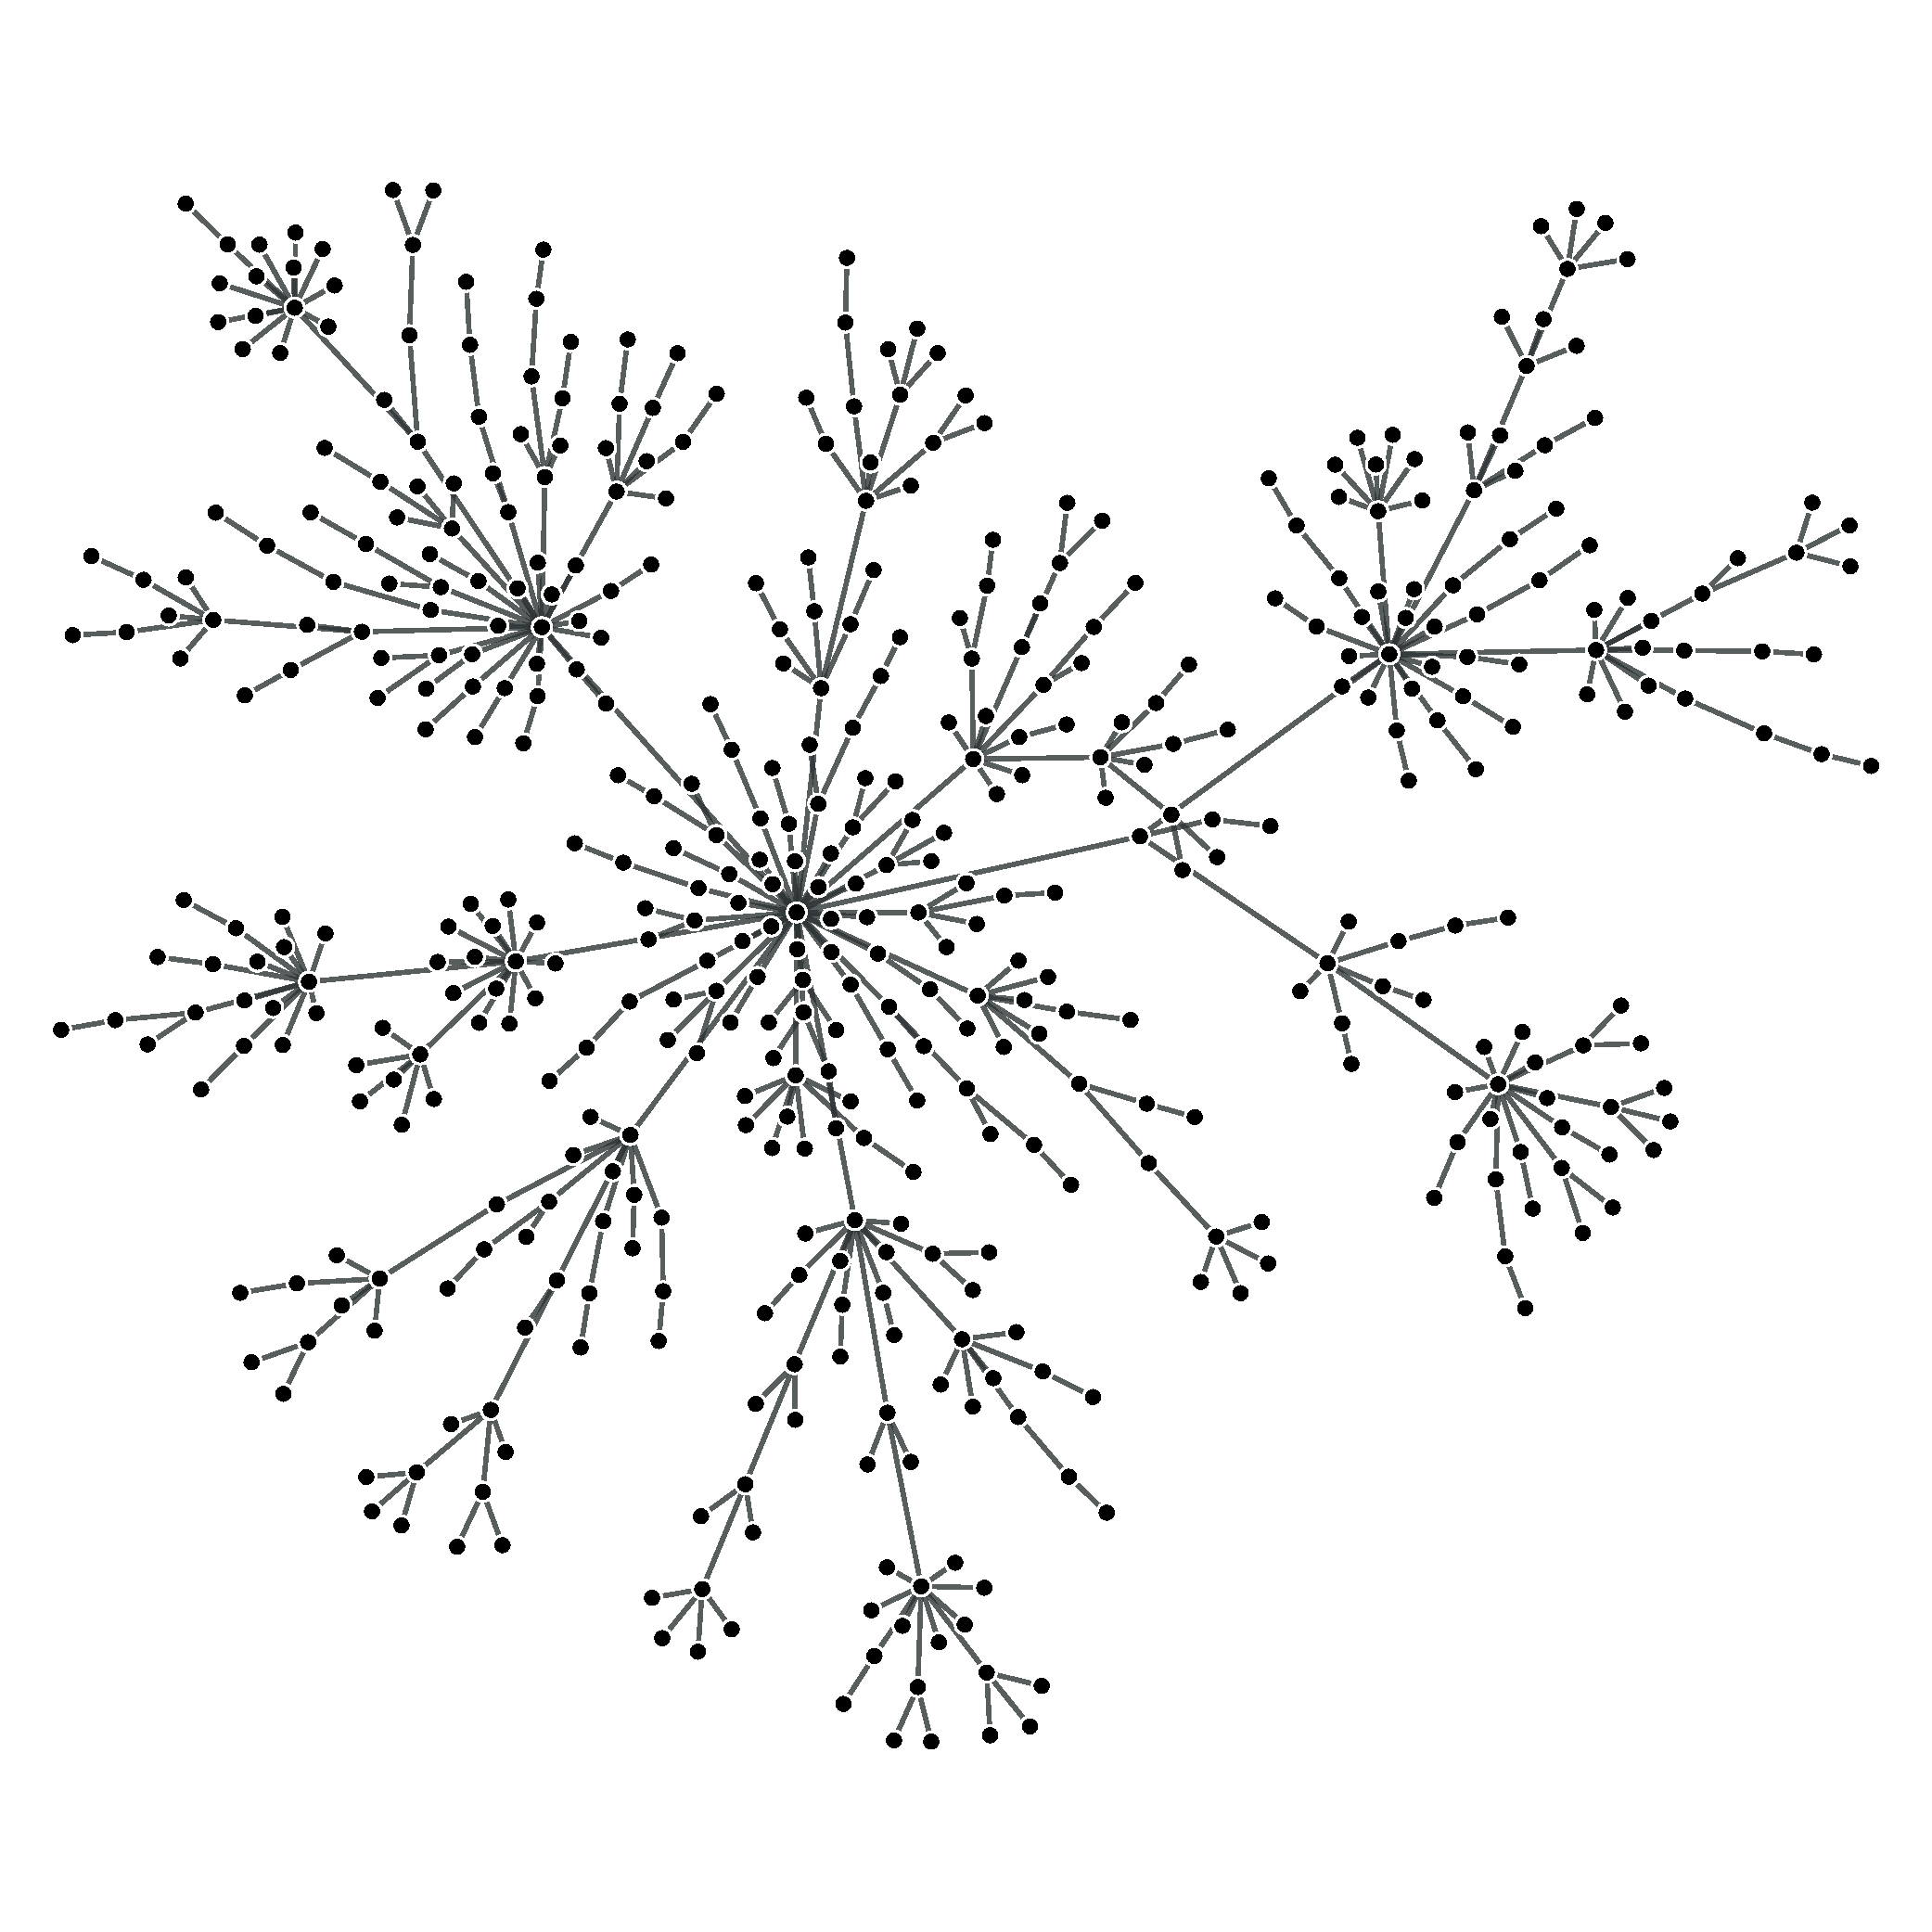
\includegraphics[width=\textwidth]{figures/GRAPHS/power-law}
 \caption{یک گراف با توزیع توانی یال‌ها
 }
 \end{subfigure}
 ~
 \begin{subfigure}[b]{0.4\textwidth}
 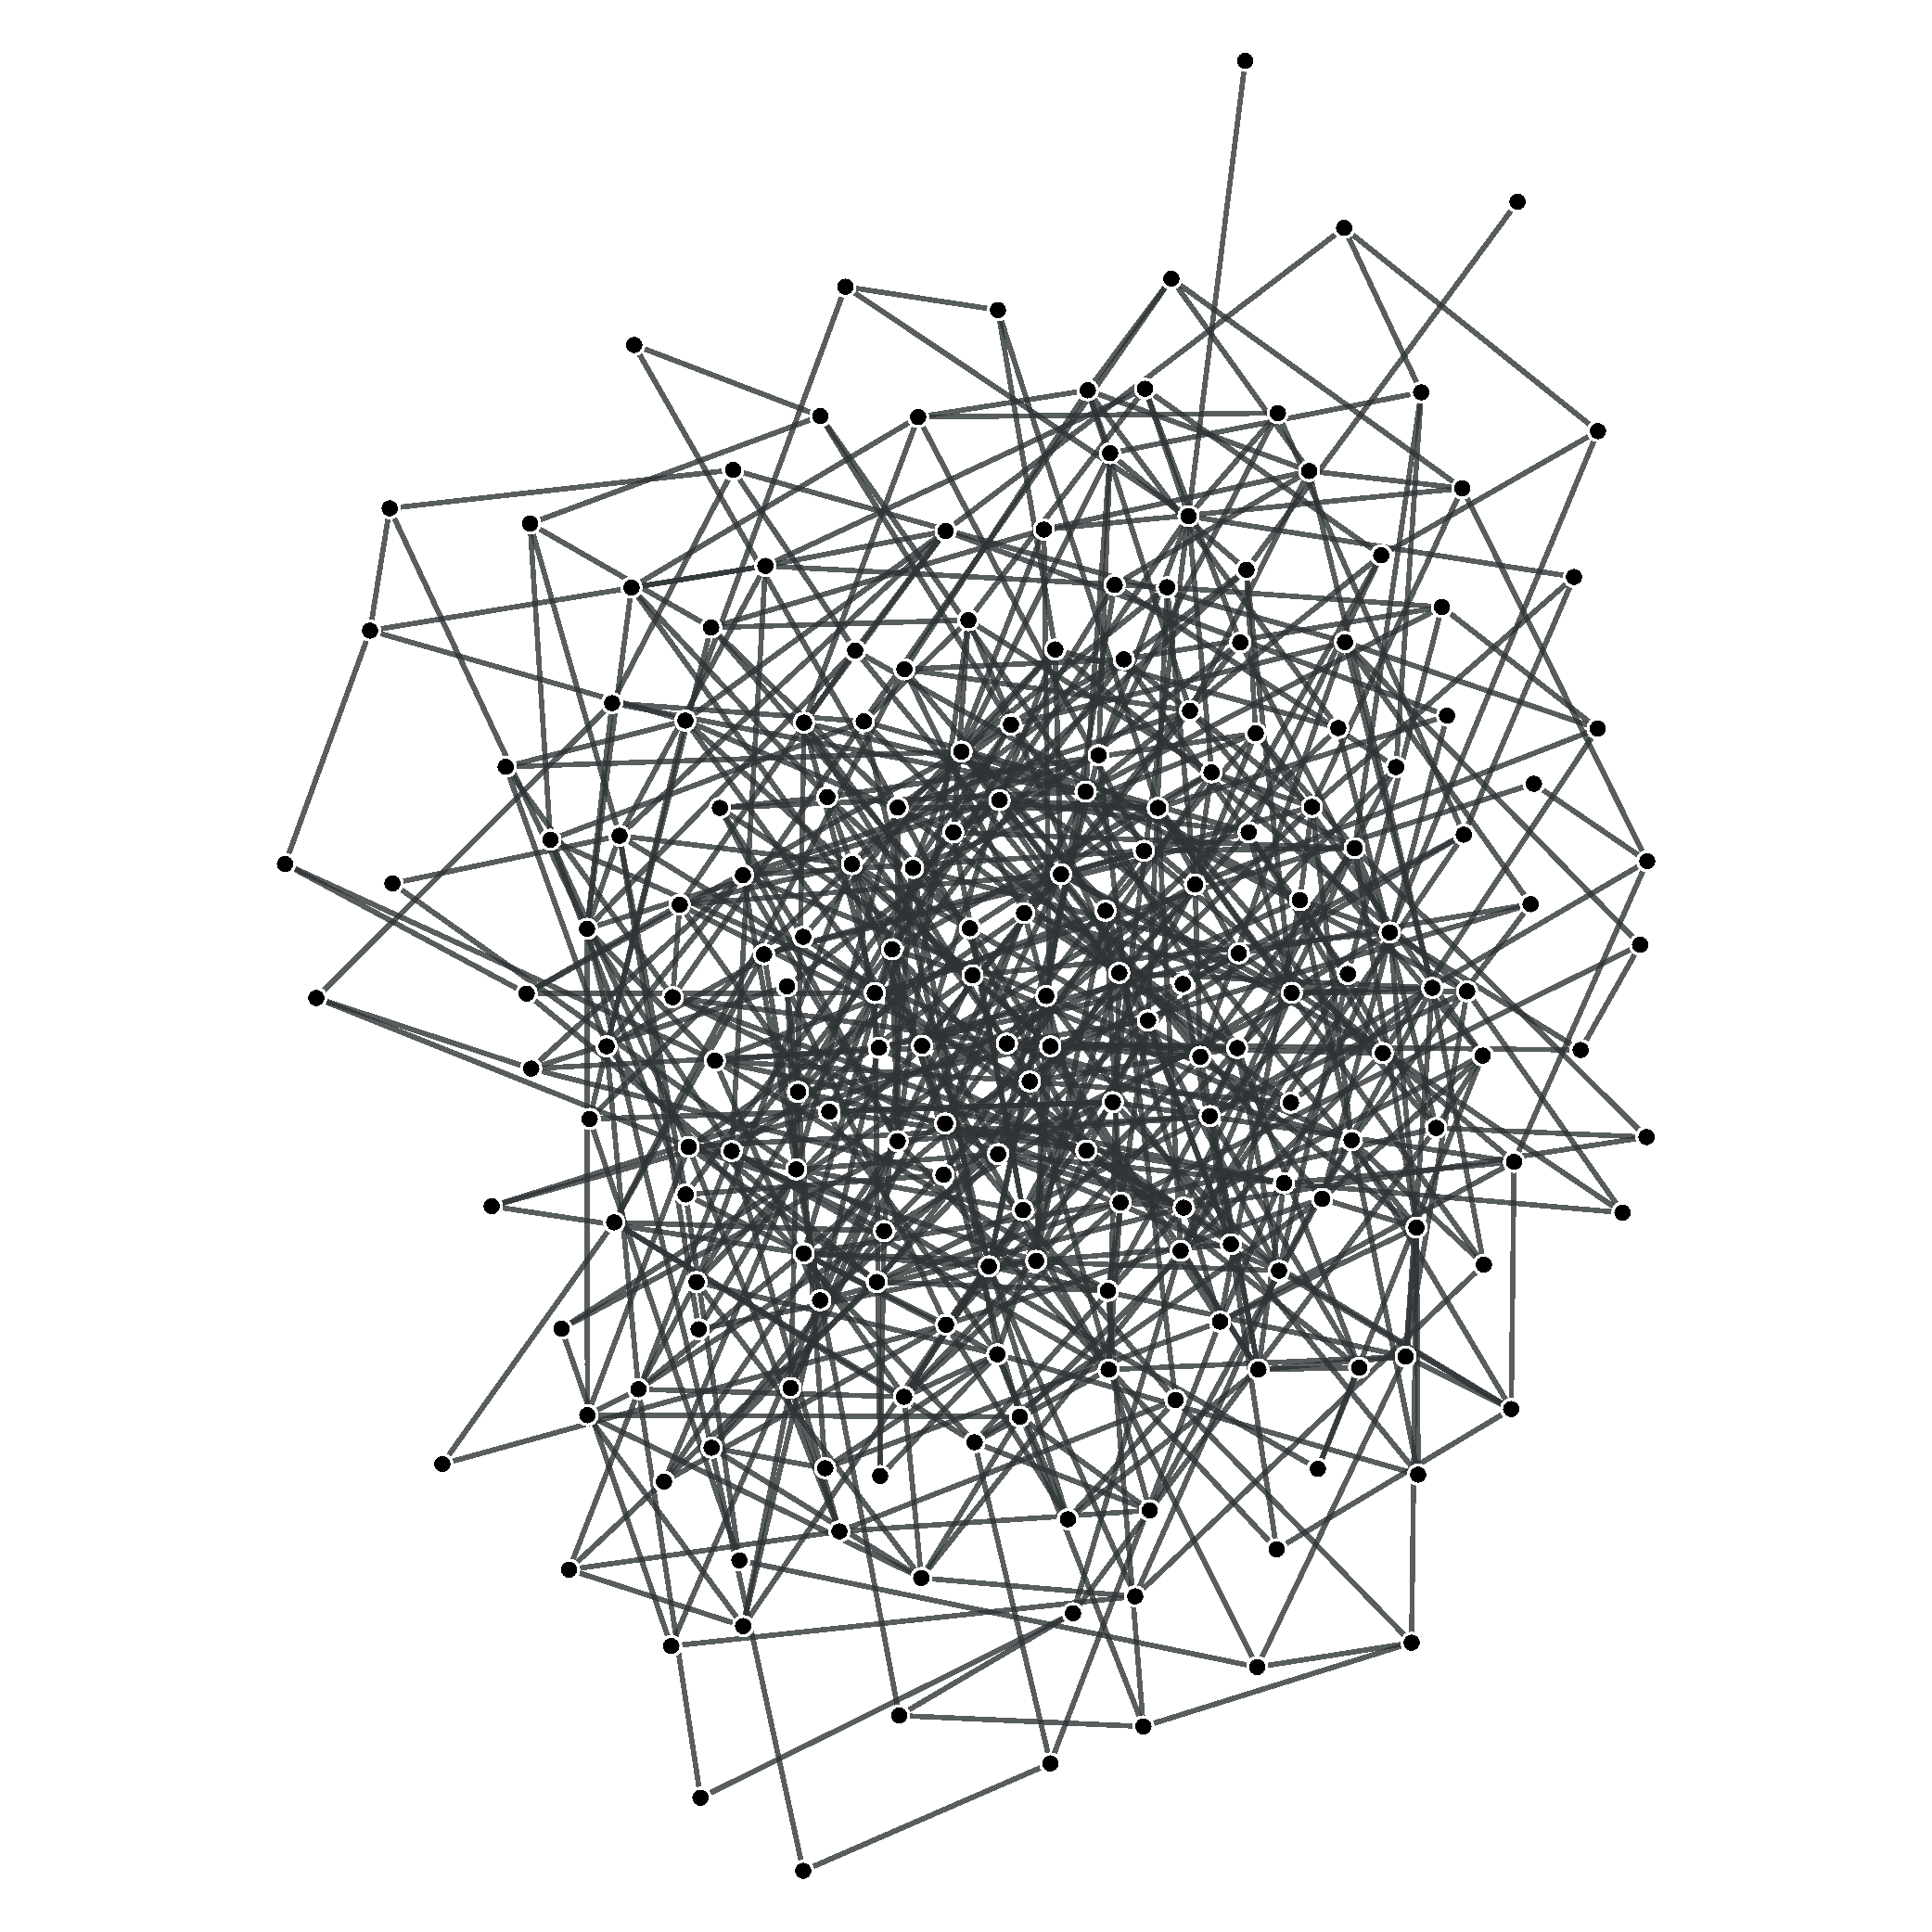
\includegraphics[width=\textwidth]{figures/GRAPHS/small-world}
 \caption{یک گراف \lr{small-world}}
 
 \end{subfigure}
 ~
 \begin{subfigure}[b]{0.58\textwidth}
 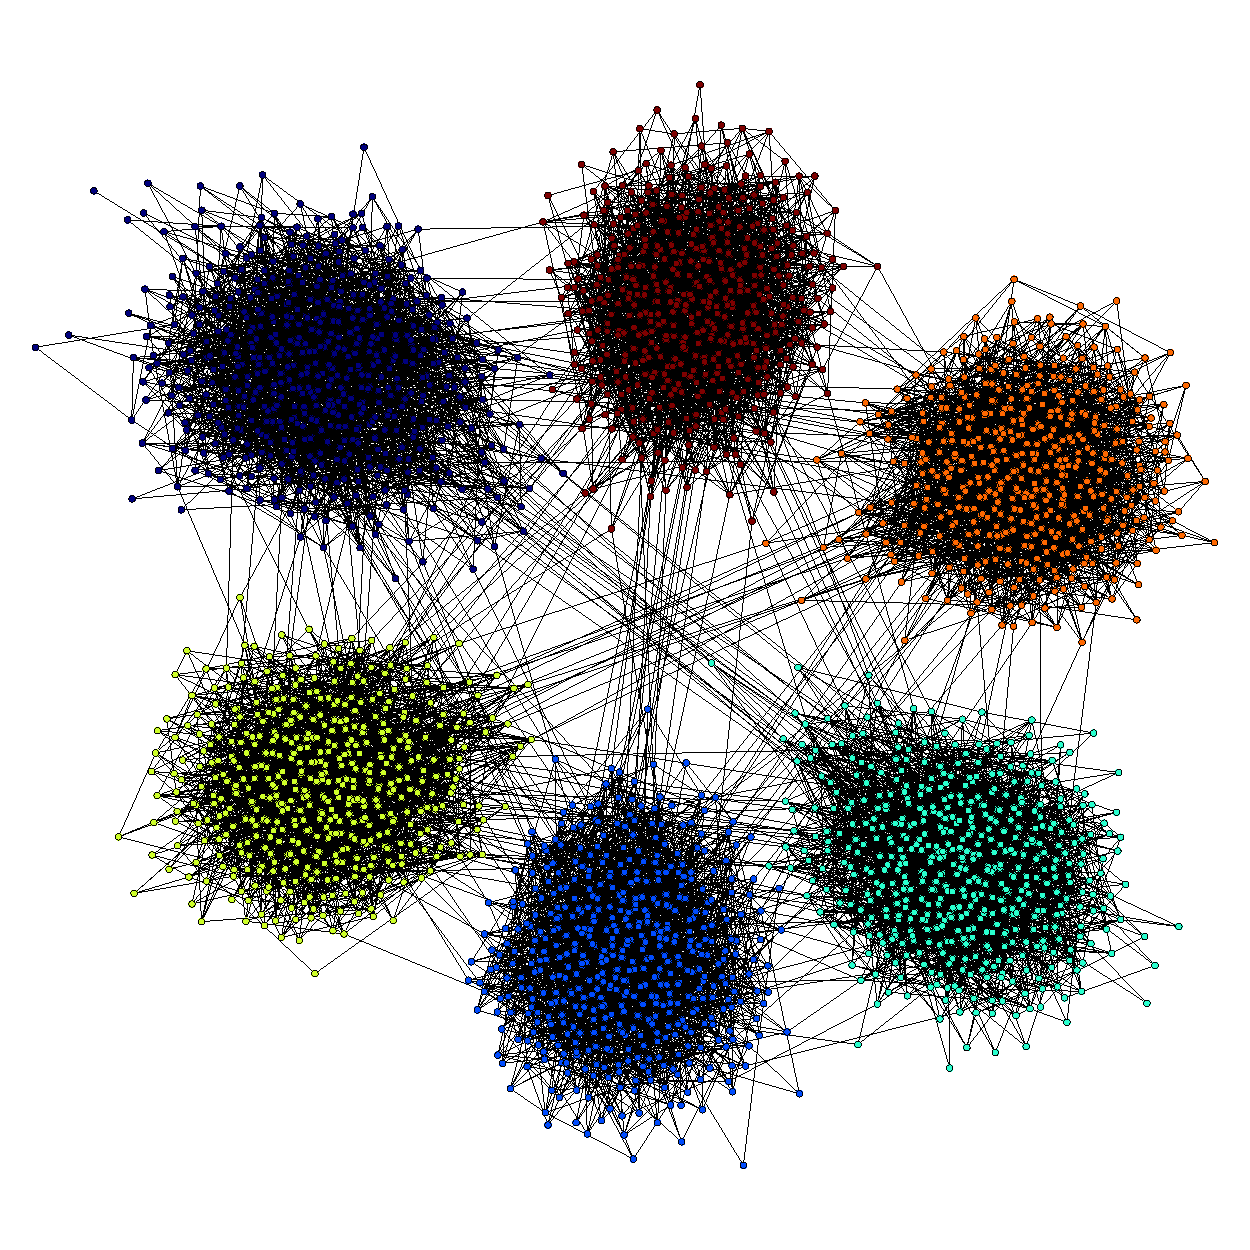
\includegraphics[width=\textwidth]{figures/GRAPHS/clusters}
 \caption{وجود خوشه‌ها‌یی از گره‌ها در گراف شبکه‌های اجتماعی}
 
 \end{subfigure}
 
 \caption[گراف شبکه‌های اجتماعی]{شکل گراف شبکه‌های اجتماعی}
\end{figure}
 
\end {persian}

%\newpage

\subsection{هوموفیلی}

\begin {persian}
\noindent
وجود هوموفیلی\پانویس {\lr{ Homophily}} میان اعضا ‌یکی از خصوصیات بنیادین شبکه‌های اجتماعی می‌باشد. هوموفیلی از طرفی به معنای شباهت ‌یک فرد با افراد مرتبط و همسایگان وی در شبکه‌ی اجتماعی مورد نظر از دید ابعاد مختلف خصوصیتی منتسب بدان فرد مثل سن و علاقه و نژاد می‌باشد \cite{sun_survey_2011}. از طرف دیگر هوموفیلی را می‌قدرت تمایل افراد جامعه به تشکیل رابطه با دیگر اعضای‌ شبیه به خودشان دانست. خصوصیات مورد بحث درباره‌ی هوموفیلی می‌قدرتند قابل تغییر(وزن و علایق) و‌ یا غیر قابل تغییر(نژاد و جنس) باشند \cite{easley_networks_2010}. وجود هوموفیلی میان اعضا به دلیل اینکه مجموعه‌ی همسایگان ‌یک فرد در ‌یک شبکه‌ی اجتماعی‌ یک مجموعه‌ی تصادفی از کل اعضای شبکه‌ی اجتماعی نیست می‌تواند ‌یک نتیجه طبیعی مقایسه‌ی فرد انتخاب شده با همسایگانش باشد \cite{sun_survey_2011}.
سه عامل زیر برای وجود هوموفیلی در شبکه‌های اجتماعی متصوراند \cite{sun_survey_2011}:

\begin{description}

\item[{تاثیر اجتماعی\پانویس {\lr{ Social Influence}}}]{: افراد تمایل دارند مانند دوستان خود رفتار کنند و این امر باعث می‌شود که در‌یک شبکه‌ی اجتماعی افراد رفتارشان تحت تاثیر همسایگانشان باشد.}

\item[انتخاب]{: افراد تمایل دارند با افرادی که از ابتدا به آن ‌‌ها شبیهند همسایه شوند.}
 
\item[متغییر‌های مخفی]{: متغییر‌های دیگری جز دو مورد فوق الذکر که در رفتار افراد جامعه تاثیر گذارند.}
 
\end{description}

 \begin{figure}[H]
 \centering
 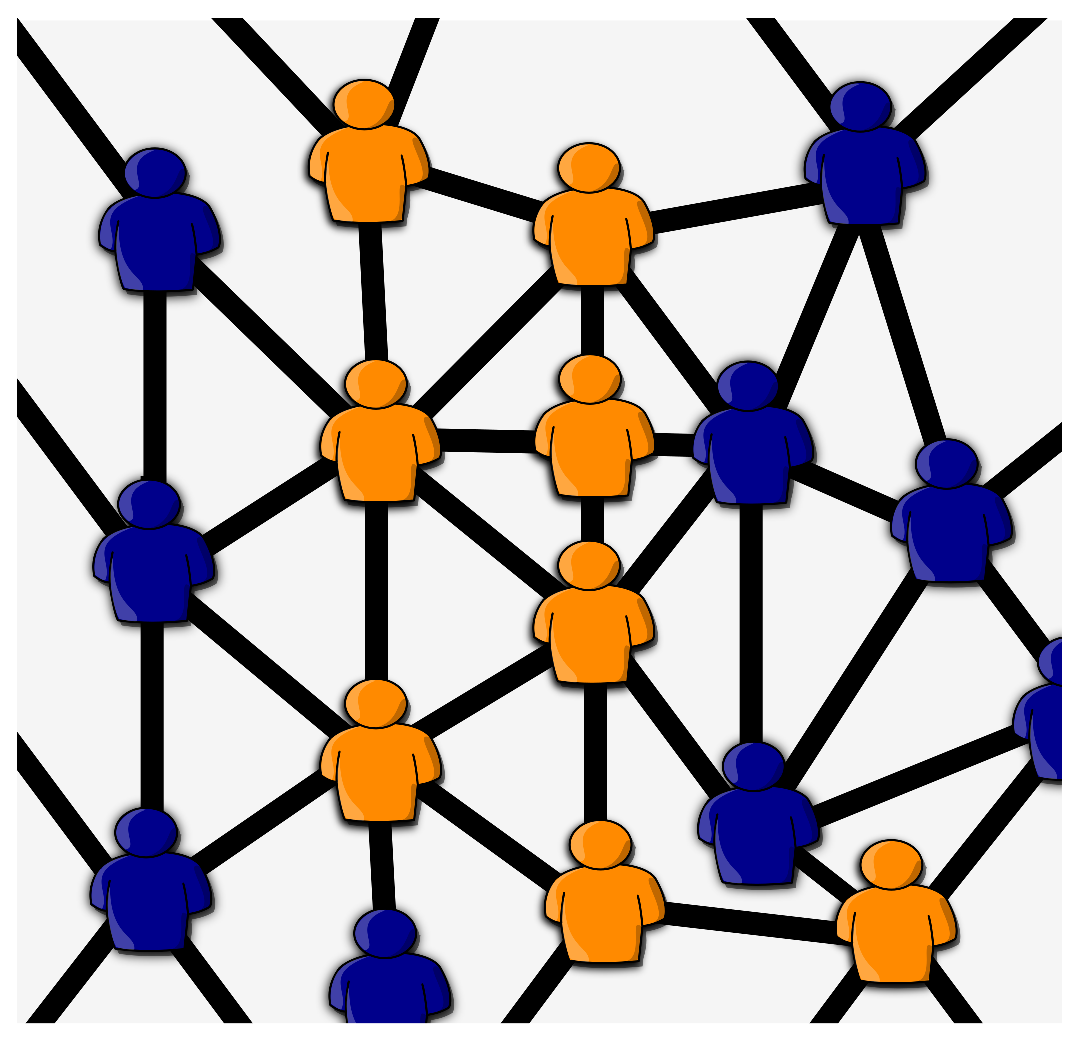
\includegraphics[scale=0.5]{figures/homophily1}
 \caption[هوموفیلی]
 {هوموفیلی: در شبکه‌های اجتماعی اکثر همسایگان و دوستان‌یک فرد دارای صفات شبیه به صفات آن فرد می‌باشند.}
\end{figure}

\indent
مقدار هوموفیلی در‌یک شبکه‌ی اجتماعی‌یک عامل مهم برای بزرگی اندازه‌ی گروه ‌‌هاست \cite{watts_six_2004} به طوری که با فرض اینکه افراد با هوموفیلی بالا معمولا تمایل زیادی با برقراری رابطه تنها با افراد شبیه به خودشان دارند، در این صورت هوموفیلی زیاد نشان دهنده‌ی گروه‌های کوچک تر و کوچکی میزان هوموفیلی نشان دهنده‌ی وجود گوناگونی در صفات همسایگان در ‌یک شبکه‌ی اجتماعی است. از طرفی‌ یکی از پیامد‌‌های پدیده‌ی پخش‌اطلاعات و نمود‌های سطح بالای آن تاثیر آن در رفتار اعضا می‌باشد. هوموفیلی به موضوع‌ یکی از موارد دخیل در شکل‌گیری و نمو گراف ساختار شبکه‌ی‌های اجتماعی که فرایند پخش اطلاعات روی آن ‌‌ها صورت می‌پذیرد مورد توجه پژوهش گران در زمینه‌ی پدیده‌ی پخش اطلاعات می‌باشد \cite{weng_role_2013}. 

\end {persian}

%\newpage
\subsection{فرضیه قدرت اتصال‌های ضعیف}
\begin {persian}
\noindent
مارک گرانوتر در سال ۱۹۷۳ نظریه قدرت اتصال‌های ضعیف\پانویس{ Strength of Weak Ties} \cite{granovetter_strength_1973} را مطرح نمود که ‌یکی از پیامد‌های آن تاکید بر تاثیری می‌باشد که اتصال‌های ضعیف و به عبارتی پل ‌‌ها\پانویس { Bridge } در گراف شبکه‌های اجتماعی در انتقال اطلاعات و تسهیل امکان ارتباط میان زیرجوامع\پانویس{ Sub-Community} جدا از هم بازی می‌کنند.\\
\indent
به زبان ساده تر بر اساس این نظریه اتصال‌های ضعیف (برای نمونه پل ‌‌ها) با اینکه قادر به انتقال حجم زیادی از اطلاعات نیستند باز نقش مهمی‌در جابجایی نوآوری و اطلاعات نوع در سطح شبکه‌های اجتماعی ایفا می‌کنند. از طرفی وجود اتصال‌های ضعیف زیاد می‌تواند به کندی فرایند پخش بیانجامد \cite{guille_information_2013,sun_survey_2011}. هم چنین بر طبق قدرت اتصال‌های اجتماعی با تعداد تکرار آن اتصال در دایره‌های اجتماعی اعضا رابطه دارد.
 \begin{figure}[H]
 \centering
 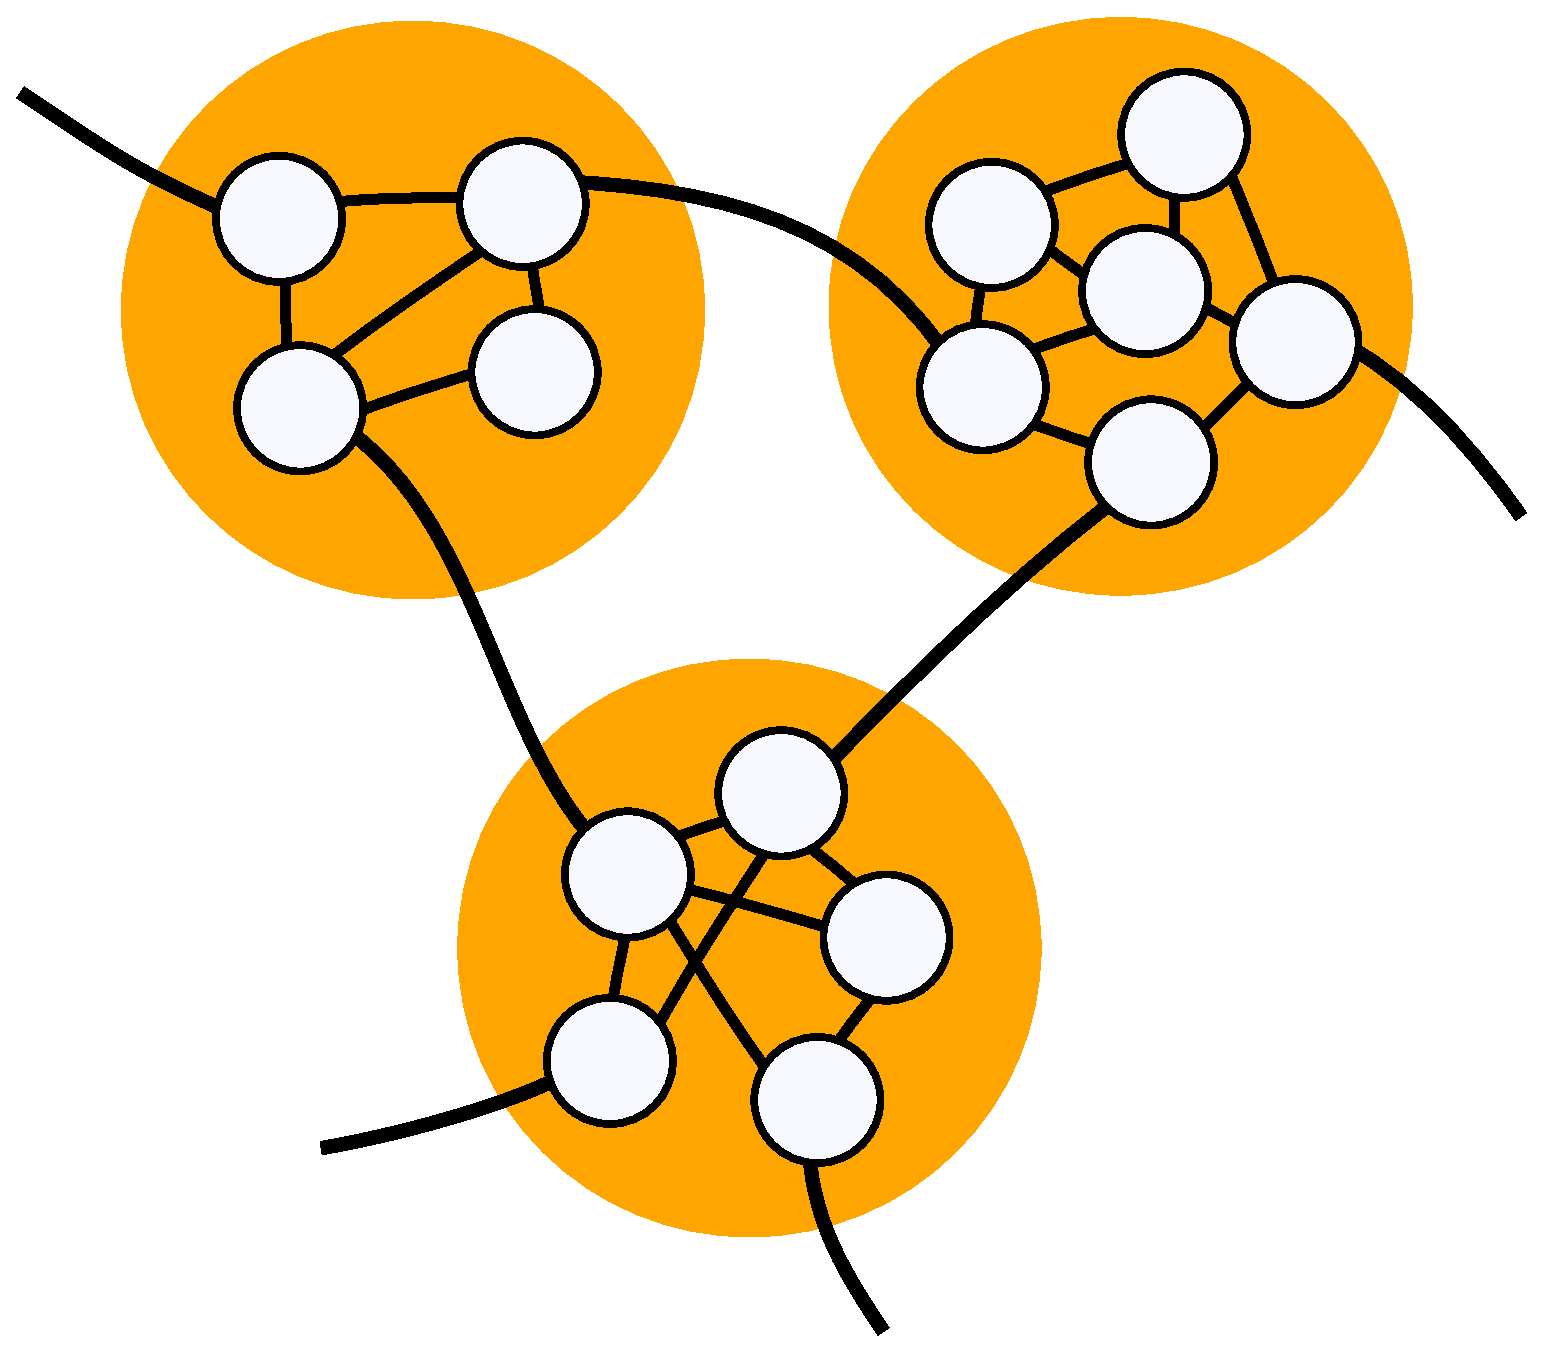
\includegraphics[scale=0.29]{figures/swt}
 \caption[فرضیه قدرت‌های ضعیف]
 {نمایی از اتصال‌های قوی(نازک تر) و ضعیف(کلفت تر) میان اعضا.}
\end{figure}


قدرت اتصال‌ها میان گره‌ها در یک شبکه‌ی اجتماعی که به صورت یک گراف مدل شده است به صورت زیر تعریف می شود.
\begin{center}
%\scalebox{1.25}
 { $ Strength_{ab} = \frac{ N(a,b) }{d(a)-1 ~+~ d(b)-1 ~-~N(a,b) } $}

\end{center}
در این فرمول $N(a,b)$ نشانده‌ی همسایه‌های مشترک گره‌های $a$ و $b$ است. $d(x)$ هم نشاندهنده‌ی تعداد یال‌های متصل به گره $x$ می باشد. برای یک گراف بی‌جهت $Strength_{ba} = Strength_{ab}$ خواهد بود.

\end{persian}

\section{فرایند پخش اطلاعات}
\begin {persian}
\noindent
فرایند پخش شدن اطلاعات به جابه جایی اطلاعات(دانش) از فردی به فرد دیگر در‌یک شبکه‌ی اجتماعی و ارتباطی اطلاق می‌شود \cite{zafarani_social_2014}. این فرایند با درنظر گرفتن زیرساخت یک شبکه‌ی اجتماعی که معمولا با یک گراف ایستا نمایش داده می شود، دارای اجزای اصلی زیر است \cite{wu_dynamics_2013}:
\begin{description}

\item[افراد]{کسانی که محتوا را تولید و مصرف می‌کنند.}

\item[محتوا]{انواع مختلف اطلاعات مثل خبر و توییت و عکس.}
 
\item[شبکه ارتباطات]{شبکه‌ی زیرین افراد و روابط آن ‌‌ها که تحت تاثیر فرایند پخش اطلاعات قرار دارد و همین طور ساختار آن این فرایند را تحت تاثیر قرار می‌دهد.}
 
\end{description}
 \begin{figure}[H]
 \centering
 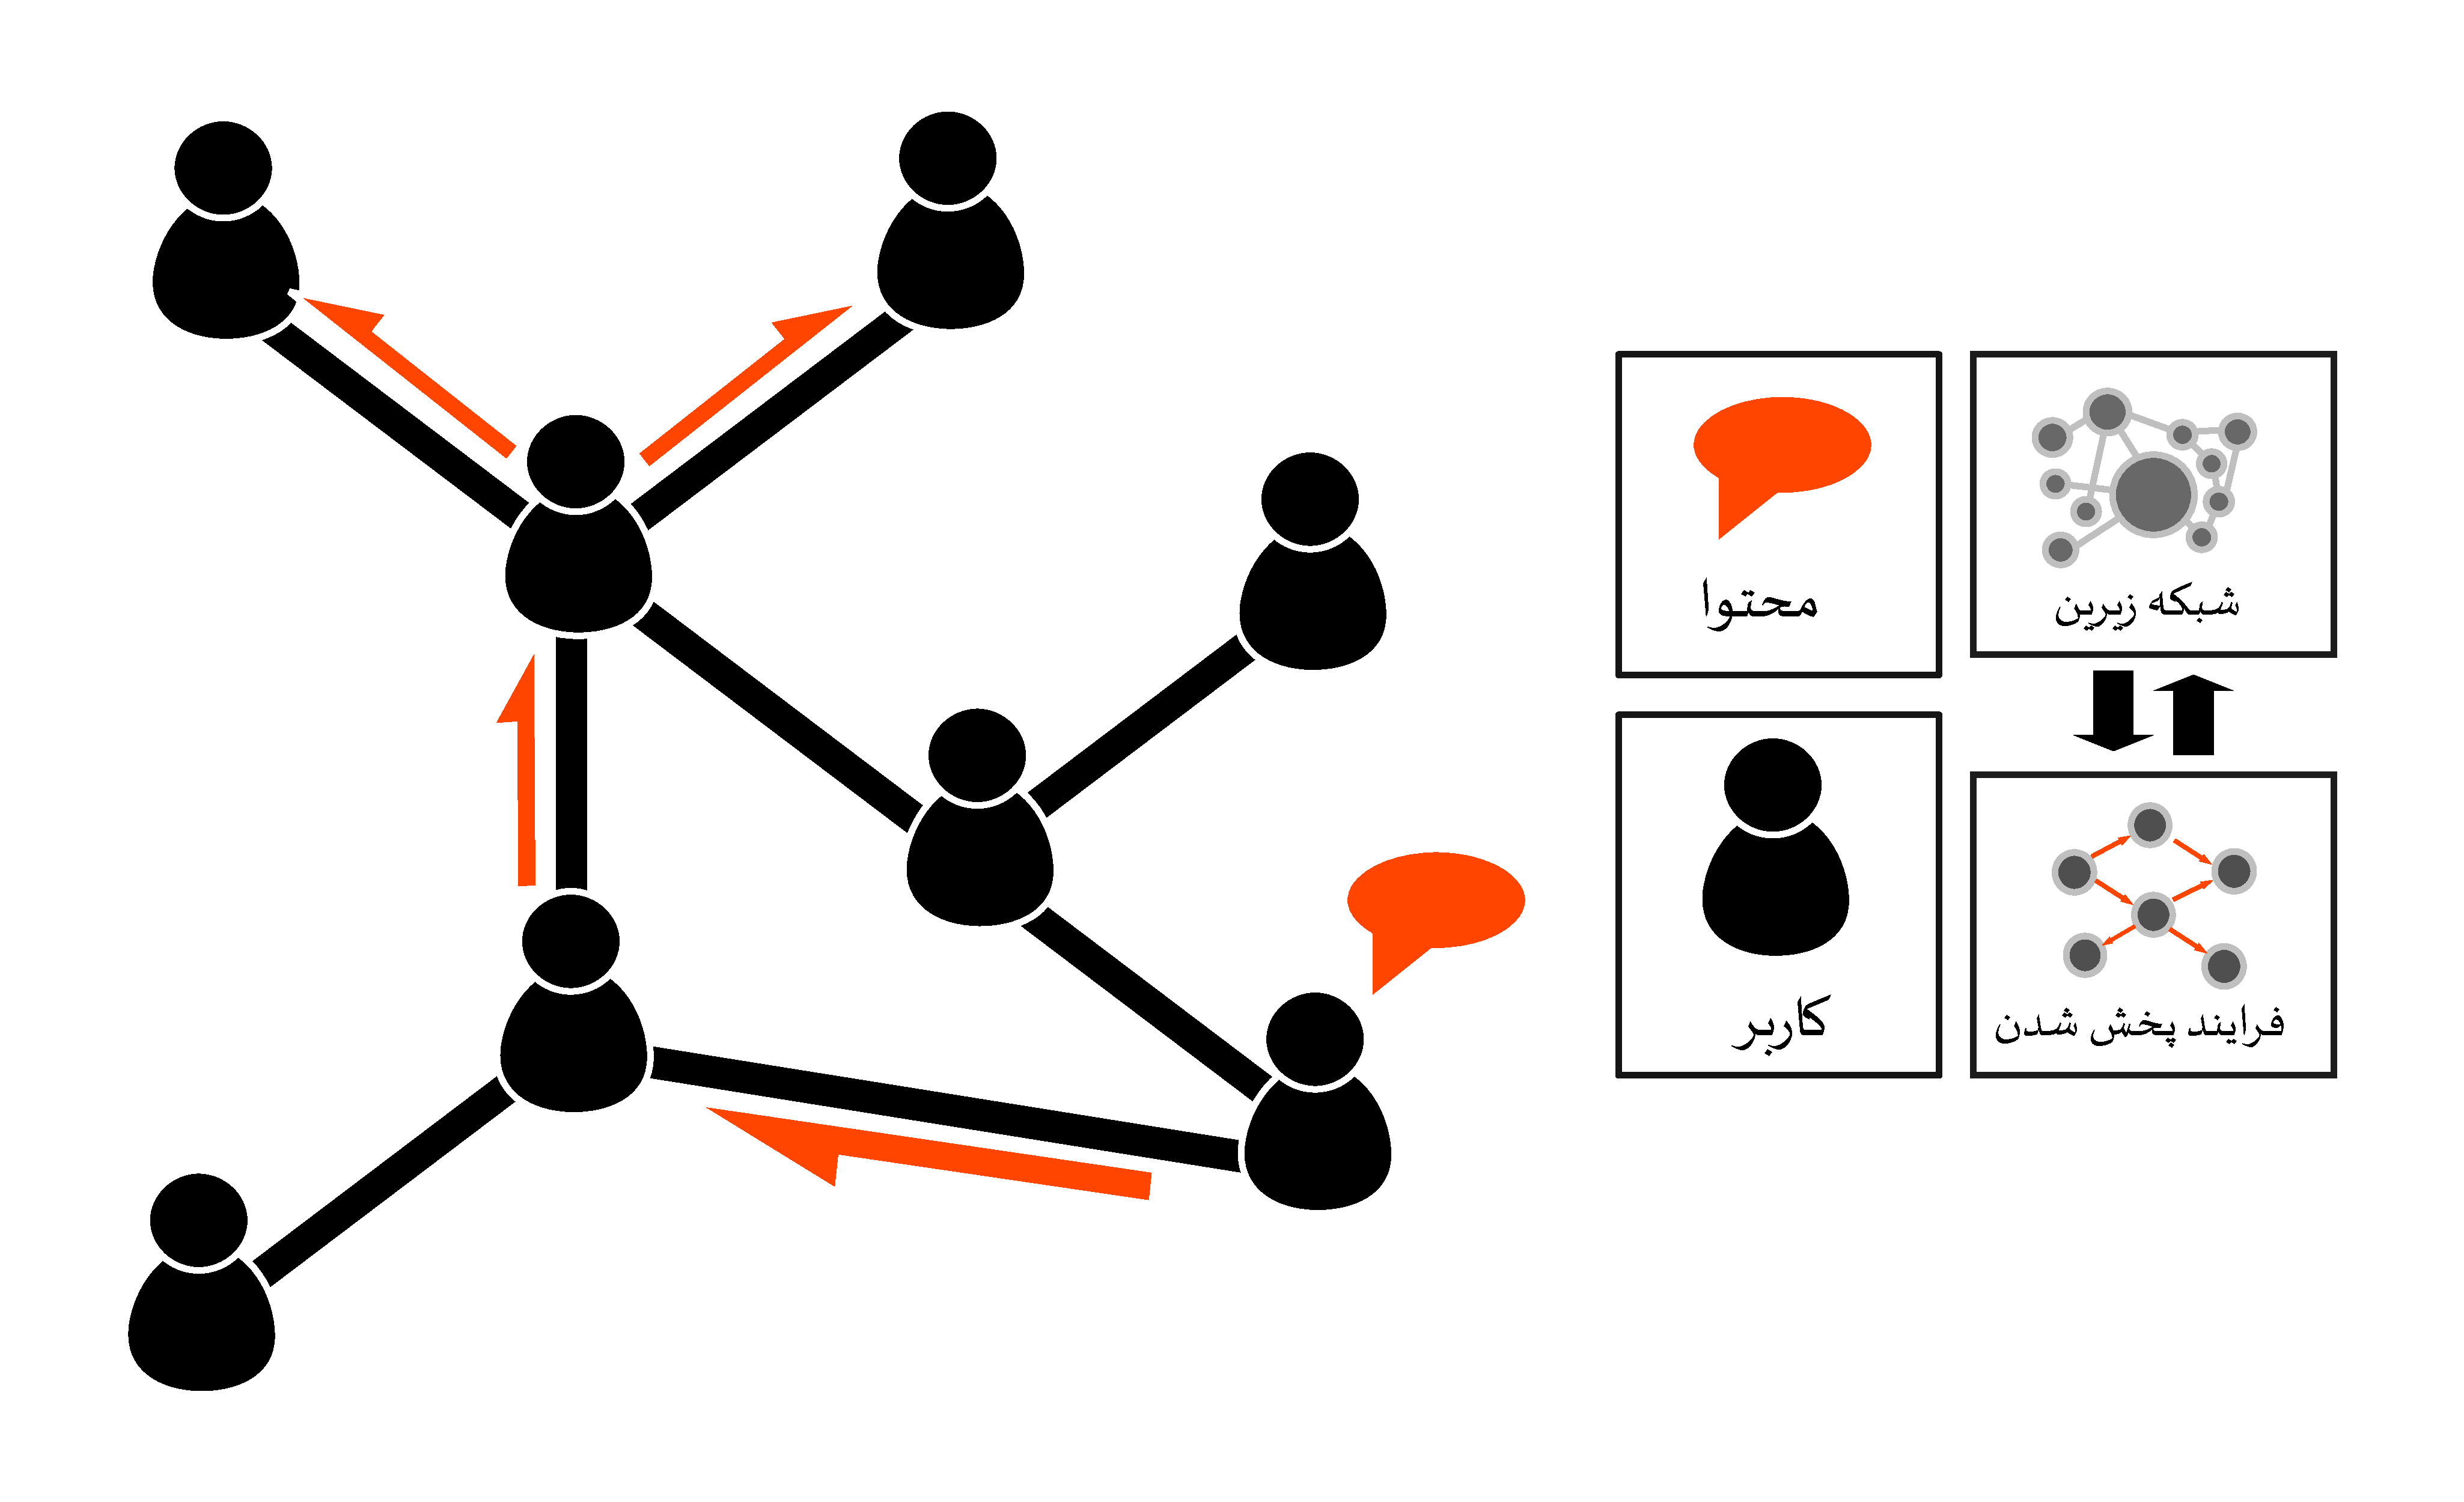
\includegraphics[scale=0.23]{figures/diffusion1}
 \caption[فرایند پخش اطلاعات در ‌یک گراف]
 {نمایی کلی از فرایند پخش اطلاعات در ‌یک گراف شبکه‌ی اجتماعی.}
\end{figure}

البته اجزای این فرایند در \cite{zafarani_social_2014} به صورتی سطح بالاتر به شکل زیر تعریف شده است:
\begin{description}

\item[فرستنده‌ها]{مجموعه‌ای معمولا کوچک از افراد که امر پخش با آن‌ها شروع می شود.}

\item[گیرنده‌ها]{مجموعه‌ای از افراد با جمعیتی بسیار زیادتر از فرستنده‌ها که محتوای فرستنده‌ها را دریافت می‌کنند.}
 
\item[ظرف]{ظرفی که محتوای اطلاعاتی مورد تبادل می‌شود. برای مثال پیام‌های یک کاربر در فیسبوک که توسط دوستانش دیده می‌شود.}

اطلاعات مورد بحث در اینجا می قدرتد یکی از موارد \textbf{شایعه} یا بکارگیری یک \textbf{تکنولوژی نوین} و یا یک \textbf{خبر} و حتی یک \textbf{تاثیر اجتماعی} که در حال فراگیری و پخش در سطح شبکه‌ی اجتماعی است باشد.
\end{description}

 \begin{figure}[H]
 \centering
 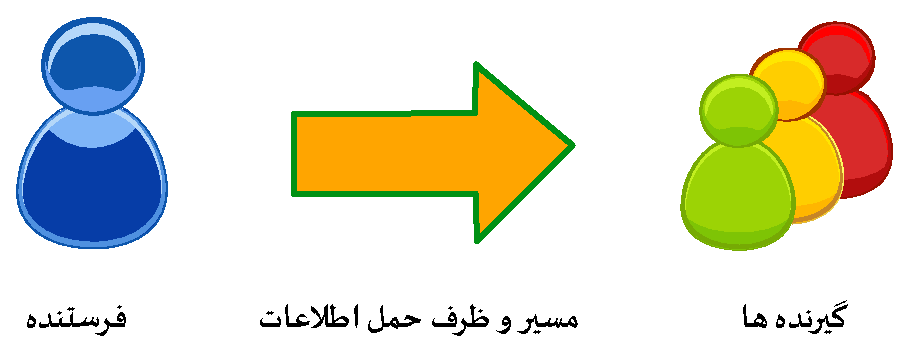
\includegraphics[scale=0.55]{figures/Diff}
 \caption[ دید کلی از فرایند پخش‌ اطلاعات]
 {نمایی کلی از پخش اطلاعات به صورت عمومی.}
\end{figure}


\end {persian}

\section{یافتن و ردیابی موضوعات مورد توجه در پخش‌اطلاعات}
\noindent {
ردیابی و شناسایی موضوعات مورد توجه در سایت‌های اجتماعی آنلاین و به طور عام سایت‌های خبری و میکروبلاگینگ\پانویس { Microblogging} مثل ارکوت\پانویس{Orkut } و توییتر معمولا در قالب شناسایی نوع موضوع شناسایی شده انجام می‌شود \cite {takahashi_discovering_2011}. 
}

\subsection{موضوع متنی}
\noindent {
در یک شبکه‌ی اجتماعی یک موضوع متنی عبارت است از یک مجموعه از عبارات مرتبط از لحاظ معنای کل که به یک مفهوم مشترک اشاره دارد \cite{guille_information_2013}.
\\
\indent
طبق این تعریف عبارت موضوع برای محتوای پیام‌های متنی تعریف شده است. از طرفی می‌قدرت این تعریف را به سه گونه تفسیر کرد:
\begin{itemize}
 \item [\textbf{الف}]
 {مجموعه‌ای از عبارات به نام $S$ و $|S|=1$}
 \item [\textbf{ب}]
 {مجموعه‌ای از عبارات به نام $S$ و $|S|>1$}
 \item [\textbf{ج}]
 {مجموعه‌ای از عبارات به نام $S$ و توزیع احتمال عبارات موجود در $S$}
\end{itemize}


}

\indent
البته باید در این جا باید متذکر شویم که فرض ما در ادامه‌ی این فصل بر این خواهد بود که منظور از عبارت موضوع همان موضوع محتوای متنی می باشد، و هر نوع موضوع مورد بحثی از این نوع است.
 \begin{figure}[H]
 \centering
 \includegraphics[scale=0.6]{figures/TOPIC}
 \caption[پیام‌های در چرخش]
 {نمایی از چرخش پیام‌ها مابین کاربران \cite{guille_information_2013}.}
\end{figure}

\subsection{موضوع‌های انفجاری}
\noindent {
موضوع‌های انفجاری\پانویس { Bursty Topics} به موضوع‌های خبری گفته می‌شود در بازه‌ی زمانی مشخصی روی رفتار کاربران سایت‌های اجتماعی تاثیر می‌گذارند و این تاثیر قابل رصد می‌باشد. خاصیت اصلی این موضوعات محدود بودن مدت زمان تاثیر آن‌ها به بازه‌ی مورد بحث است به طوری که پیش از شروع زمان بازه و همین گونه پس از آن اثری از رابطه‌ی موضوع و تاثیر آن زیاد به چشم نمی‌آید \cite{guille_information_2013}. همه‌‌ی کار‌های انجام گرفته در این زمینه درباره‌ی شناسایی و ردیابی موضوعات برای داده‌ی متنی محض می باشد.
\\
%\indent

 \begin{figure}[H]
 \centering
 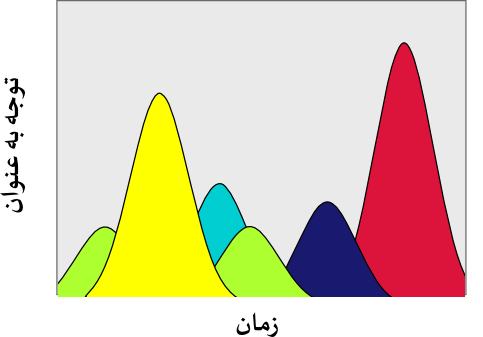
\includegraphics[scale=0.6]{figures/others/BT}
 \caption[موضوع‌های مهم]
 {نمایی از میزان توجه به موضوعات مهم که فرایندی انفجاری را نشان می دهد \cite{guille_information_2013}.}
\end{figure}

 \begin{figure}[H]
 \centering
 
\includegraphics[scale=0.5]{figures/others/fifa15}
 \caption[خبر انتشار بازی میان کاربران سایت تورنت]
 {نمایی از \lr{WordCloud} کلماتی که کاربران سایت
 \href{https://kickass.to/fifa-15-ultimate-team-edition-sc-t9600660.html\#comment}{\lr{KickAss.to}}
 با هم درباره‌ی بازی \lr{Fifa 15} از تاریخ ۱۸ سپتامبر تا ۵ اکتبر ۲۰۱۴ رد و بدل نموده اند.
 }
\end{figure}


}

\section{ محدودیت در توجه و اقتصاد توجه}
\begin {persian}
\noindent
بر طبق نظریه دانبر \cite{dunbar_social_1998}‌یک انسان امروزی قادر به برقراری رابطه اجتماعی پایدار با تعداد معدودی از دیگر اعضای جامعه می‌باشد. از طرفی بر طبق نظریه اقتصاد توجه که توسط سیمون \cite{lilian_weng_information_2014,simon_designing_1971} مطرح شده است حجم زیاد اطلاعات نیازمند(همان مقدار) توجه می‌باشد، حجم این اطلاعات(موجود در شبکه‌های اجتماعی آنلاین) بسیار بیشتر از قدرت توجه و دریافت افراد این جوامع می‌باشد. برای نمونه شبکه‌های اجتماعی آنلاین مانند توییتر که کاربران آن داده‌های بسیار زیاد و متنوعی را در قالب پیام‌های بسیار فشرده تولید می‌کنند.‌ یکی از موارد مهمی‌ که از دو مورد مطرح شده برداشت می‌شود وجود محدودیت برای توجه به محتوای موجود در سایتی مثل توییتر است. چنین فرضی در مطالعه چگونگی فرایند پخش اطلاعات در سطح شبکه‌های اجتماعی آنلاین مورد توجه می‌باشد.

\end{persian}


\section{میم}
\begin {persian}
\noindent
میم\پانویس { Meme } به معنی ایده و‌ یا رفتار و‌ یا همین‌گونه منشی است که در‌ یک فرهنگ از فردی به فرد دیگر قابل انتقال و سرایت است \cite{blackmore_meme_2000}، به زبان ساده تر همان گونه که ژن‌ها واحد انتقال خصایص ‌یک موجود زنده به فرزندانش هستند میم هم واحد انتقال مفاهیم و ایده‌‌ها و رفتارها در فرهنگ‌های حاکم در جوامع انسانی می‌باشد. ریچارد داکینز اولین بار این مفهوم را در کنار مفهوم تکامل و انتقال خواص ژنتیک از نسلی به نسل بعد به خاطر شباهت بین این دو مورد، به کار برده است \cite{dawkins_selfish_1976}. 
\\
\indent
با توجه به گوناگونی زیاد نوع‌های رسانه‌های آنلاین و نیاز‌ به مفهومی‌ خنثی از محتوای رسانه‌های اجتماعی آنلاین میم در تحقیق در زمینه‌های چگونگی انتشار و پخش افکار و اطلاعات در سطح شبکه‌های اجتماعی آنلاین مورد توجه می‌باشد، برای نمونه 
% no spaces between citations is allowed
\مرجع{bonchi_meme_2013, wei_competing_2013, massad_modelling_2013, weng_predicting_2014, weng_competition_2012}. 


\end{persian}

%\subsection{سرایت و تقلید}

\section{خلاصه‌ی مطالب فصل}
\noindent 
در این فصل در ابتدا شبکه‌‌های اجتماعی و موارد مهم مربوط به این شبکه‌ها از قبیل هوموفیلی و فرضیه اتصال‌های ضعیف به همراه موضوع و نوع انفجاری آن تعریف و توضیح داده شدند. همین طور نشان دادیم که برای مدل‌سازی این شبکه‌ها از نظریه گراف‌ها استفاده می‌شود. هم‌چنین دو تعریف برای فرایند پخش اطلاعات ارایه شد که در پی آن‌ها مفهوم‌های میم و اقتصاد توجه به موضوع بعضی از عناصر تاثیر گذار در فرایند پخش اطلاعات معرفی شدند. 

\chapter{مدل‌سازی پخش‌اطلاعات در شبکه‌های اجتماعی آنلاین}
\newpage
\begin{persian}
\section {مقدمه}
\noindent
در این فصل به معرفی مدل‌های مطرح شده برای فرایند پخش اطلاعات خواهیم پرداخت. در ادامه توضیحی مختصر برای تک تک این مدل‌ها به همراه‌یک طبقه بندی براساس خصوصیات مدل‌های مورد نظر ارایه شده است. سرانجام مدل‌های معرفی شده را مقایسه می‌کنیم و سرانجام هم ارجاع‌های لازم برای مطالعه بیشتر برای انواع مدل‌های مشتق شده از مدل‌های اولیه و اصلی داده خواهند شد. ضمنا در این فصل کلمات گره و رأس و همین‌طور یال و اتصال دو به دو مترادف هم می‌باشند.
%\newpage
\section {مدل‌های پخش اطلاعات}
\noindent
در گذشته از مدل‌های همه گیری مریضی‌های مسری مانند سل برای مدل سازی فرایند پخش اطلاعات در سطح شبکه‌های اجتماعی استفاده شده است \cite{watts_six_2004,easley_networks_2010}. در سال‌های اخیر مدل‌های مانند مدل انتشار مستقل\پانویس{\lr{ Independent Cascading Model}} 
و مدل آستانه خطی\پانویس {\lr{ Linear Threshold Model}}
در زمینه بررسی الگوریتمیک فرایند پخش به این دسته از مدل‌ها اضافه شده اند. دو مدل \lr{LT} و \lr{IC} به صورت امروزی نخستین بار در \cite {kempe_maximizing_2003} برای بررسی مسئله‌ی حداکثر سازی تاثیر اجتماعی افراد یک شبکه‌ی اجتماعی برای پذیرفتن و ترویج نوآوری پیشنهاد شده اند.
این دو مدل و همین‌طور مدل‌های همه گیری جزو مدل‌های اصلی فرایند پخش اطلاعات می‌باشند که مشتقات زیادی برای آنان ارایه شده است. هم چنین مدل‌هایی براساس نظریه بازی‌ها\پانویس {\lr{ Game Theoric Models}} \cite{jiang_evolutionary_2013} و همین طور مدل‌هایی بر پایه زنجیره‌های مارکوف پیوسته زمان برای مدل سازی و بررسی فرایند پخش اطلاعات پیشنهاد شده اند، که در بخش پایانی این فصل ارجاع‌های مربوط به این مدل‌ها برای مطالعه‌ی بیشتر خواننده داده شده است. 
\\


%\newpage
\section{مدل‌های انتشار}
\noindent
{
در این بخش به معرفی و تشریح مدل‌های انتشار مطرح برای مدل‌کردن فرایند پخش اطلاعات می‌پردازیم. 
}
\subsection{مدل انتشار مستقل}
\noindent
{
مدل انتشار مستقل جزو دو مدل اصلی و مطرح برای مدل‌سازی فرایند پخش اطلاعات در سطح شبکه‌های اجتماعی است. ریشه‌ی این مدل به مدل‌های حرکت ذرات در فیزیک باز می‌گردد \cite{chen_scalable_2010}. به طور کلی این مدل و مشتقات آن‌ها برای مدل سازی پذیرش و استفاده‌ی چیز‌های جدید و تاثیرگذار در بستر شبکه‌های اجتماعی به کار رفته شده اند. در این مدل بستر پخش اطلاعات یک گراف جهت‌دار ایستا $G =(V,E)$ در نظر گرفته می‌شود که $V$ و $E$ به ترتیب مجموعه‌های گره‌ها و یال‌های $G$ می‌باشند. هر اتصال یعنی وجود یک یال جهت دار از گره $n$ به گره $x$ در این شبکه به صورت $e=(n,x)$ که $n \neq x$ تعریف می‌شود.
برای هر گره‌ مانند $n$ مجموعه‌ی فرزندان $n$ یا $C_n$ به صورت $C_n = \{x; x \in (n,x)\}$ تعریف می‌شود و همین‌طور تابع والدین $n$ هم به نام $H_n$ به صورت $W_n =\{x; x \in (x,n)\}$ تعریف می‌شود. \\
\indent
در این مدل در ابتدا به هر یال جهت دار $e$ عدد مثبت $p_{nx}$ با شرط $0 < p_{nx} < 1$ نسبت داده می‌شود. به $p_{nx} $ احتمال پخش $(n,x)$ هم گفته می‌شود. فرایند پخش با انتخاب یک مجموعه‌ی آغازین به نام $D(0)$ از گره‌های شبکه‌ی مورد مطالعه شروع می‌شود، بدین صورت که با فرض این امر که در اینجا نیز هر گره می‌تواند در یکی از دو حالت فعال و یا غیر فعال باشد، گره‌هایی که در $D(0)$ قرار دارند در حالت فعال فرض می‌شوند و در هر گام زمانی $t=\{0,1,..,w\}$ یک گره فعال مانند ‌$n$ می‌تواند هر گره فرزند غیر فعال خود مانند $x$ را با احتمال $p_{nx}$ فعال کند. باید توجه داشت در صورتی که چند گره والد گره‌ای مانند $n$ در گام $t$ فعال باشند ترتیب اعمال احتمال فعال سازی $n$ توسط یکی از آن‌ها به صورت اختیاری و بدون در نظر گرفتن اولویت خاصی در نظر گرفته می‌شود و تنها امر مهم این است که فعال سازی برای $n$ از طرف گره‌های والدش باید همگی در گام $t$ انجام پذیرد. ضمنا در این مدل جدا از فعال شدن و یا فعال نشدن گره فرزند در گام $t$ هر گره والد تنها یک بار فرصت فعال سازی گره فرزند خود را دارد. اجرای فرایند انتشار مستقل وقتی دیگر گره‌ای را نتوان 
فعال کرد خاتمه می‌یابد.
در زیر تابع فعال سازی و مجموعه‌ی $\theta$ برای یال دلخواه $e$ را مشاهده می‌کنید.

\centerline{
\scalebox{1.25}{
 \begin{latin}
 $ Y_1(e_i) = p_{e_i} ; \theta =\{p_{nx}; (n,x) \in E\} $
 \end{latin}}}

به کمک مجموعه‌ی $\theta$ می‌توان تابع درجه تأثیر گذاری هر گره‌ یا تعداد گره‌های فرزند گره مورد بحث را که احتمال می‌دهیم در گام بعدی فعال باشند به صورت زیر تعریف کرد.

\centerline{
\scalebox{1.25}{
 \begin{latin}
 $ Y_2(n)=\mu(n,\theta)$
 \end{latin}}}

در اینجا یکی از موارد مهم یافتن آن دسته از گره‌های فعال اولیه خواهد بود(به طور دقیق‌تر $k$ تا گره) که با انتخاب به عنوان مجموعه‌ی گره‌های فعال اولیه، حداکثر پخش اطلاعات را با استفاده از این مدل حاصل می‌آورند. اگر بخواهیم$\mu(n,\theta_0)$ را برای رتبه بندی گره‌ها برای امر ذکر شده محاسبه کنیم، با فرض اینکه$\theta_0$ نشاندهنده‌ی مجموعه‌ی واقعی احتمال‌های پخش برای کل شبکه‌ی ما می‌باشد چون مجموعه‌ی $\theta_0$ را نمی‌توان در اکثر اوقات پیدا کرد می‌توان به‌جای $\mu(n,\theta_0)$ میزان $\mu(n,\hat{\theta})$ را برای گره‌های اولیه محاسبه برای رتبه دهی گره‌ها از نظر تأثیر گذاری روی فرایند پخش اطلاعات محاسبه نمود. در اینجا $\hat{\theta}$ مجموعه احتمالاتی است که به صورت تجربی و تقریبی برای گره $n$ پیدا شده است.



 \begin{figure}[H]
 \centering
 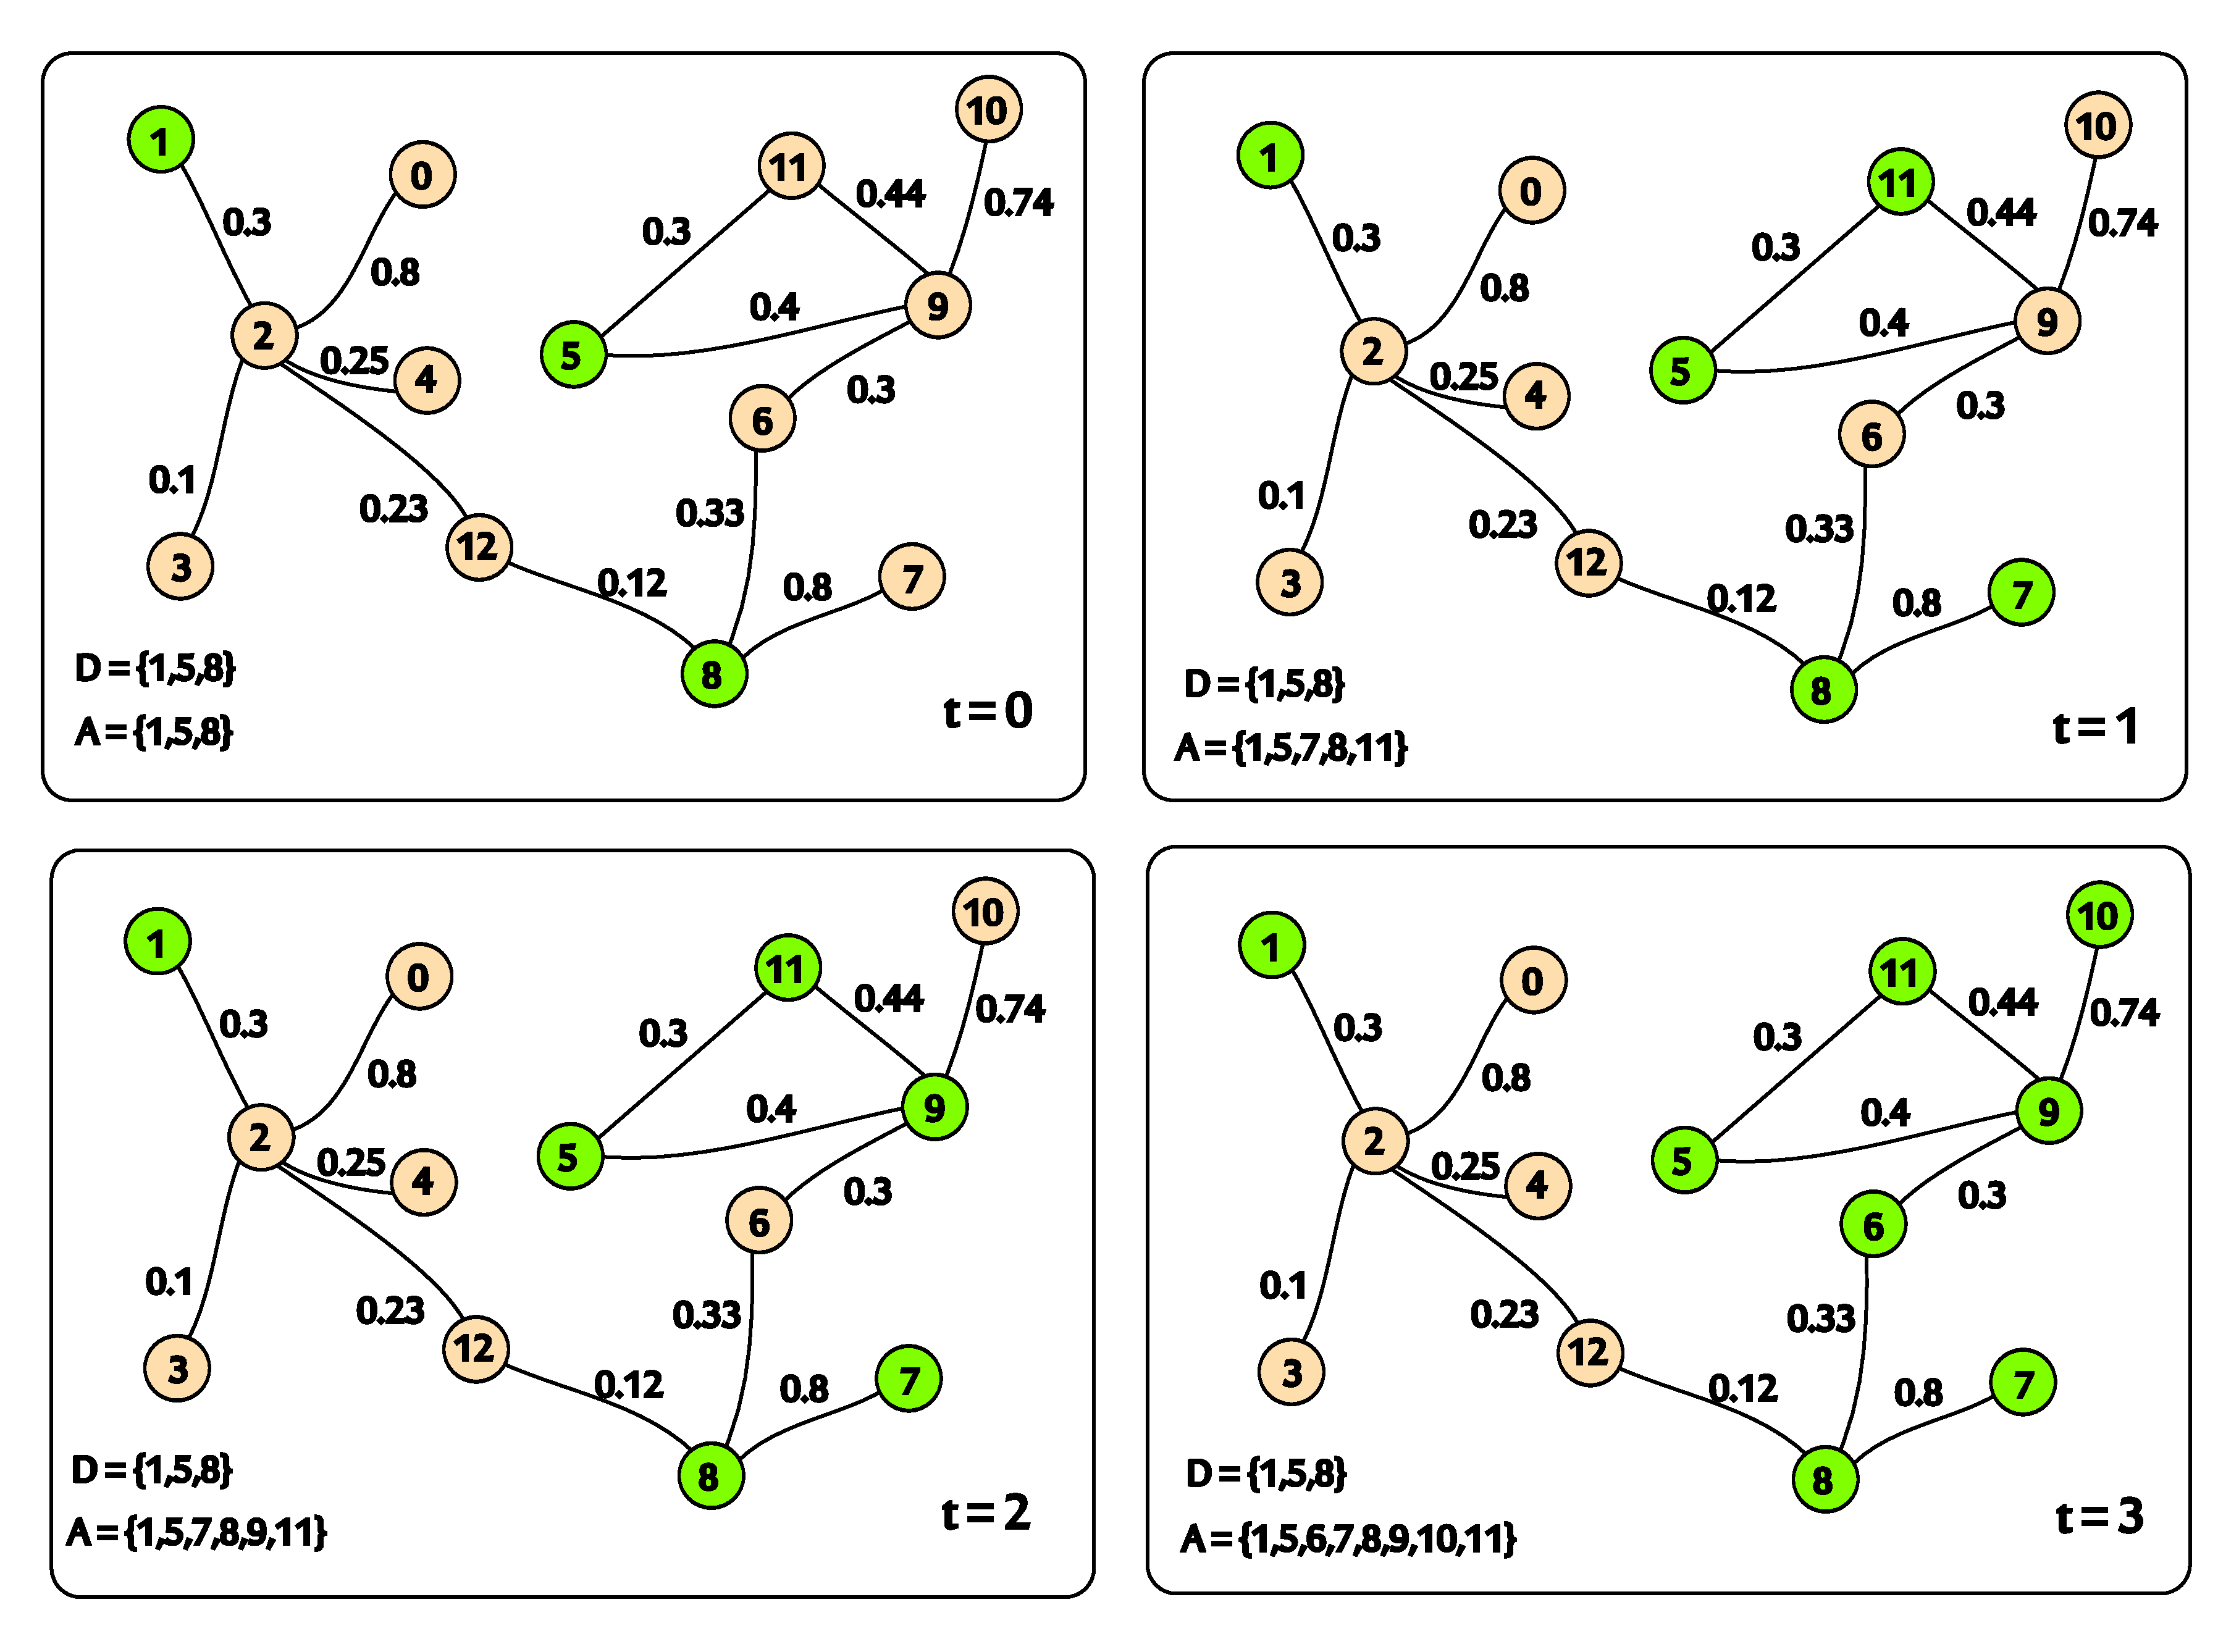
\includegraphics[scale=0.24]{figures/icm}
 \caption[مدل انتشار مستقل]
 { شبیه سازی فرایند کار مدل انتشار مستقل با ۳ گره فعال اولیه.}
\end{figure}

 \begin{figure}[H]
 \centering
 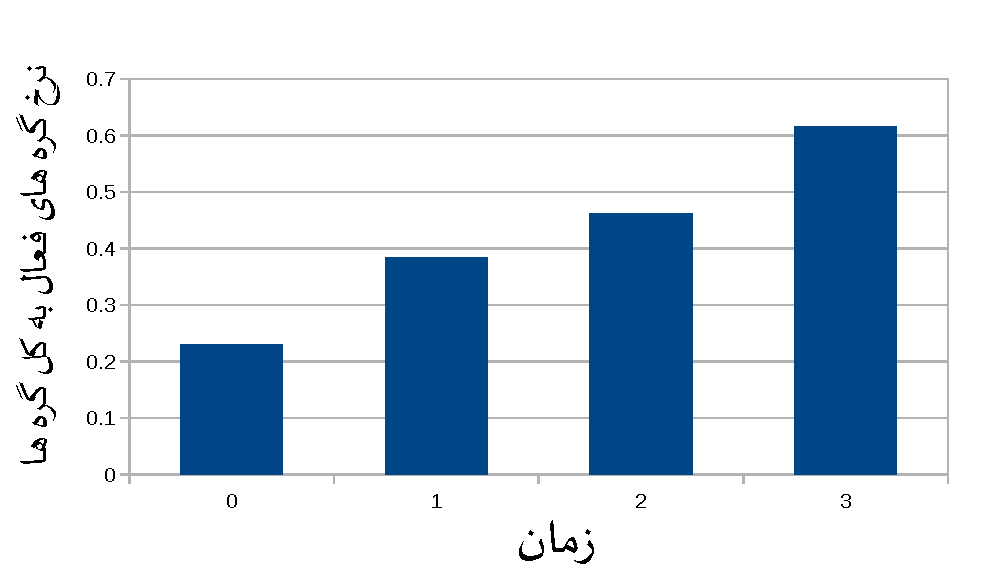
\includegraphics[scale=0.6]{figures/icm_chart1}
 \caption[شبیه سازی مدل انتشار مستقل]
 {روند پخش در حین شبیه سازی فرایند کار مدل انتشار بالا.}
\end{figure}


}

\subsection{مدل انتشار کاهشی}
\noindent{
 مدل انتشار کاهشی\پانویس { Decreasing Cascade Model} در مقایسه با مدل انتشار مستقل عملی تر و عمومی تر می‌باشد. در این مدل اگر $S$ نشان دهنده‌ی مجموعه‌ی گره‌هایی باشد که در گذشته سعی در فعال سازی گره $v$ نموده اند ولی موفق به این کار نشده اند باشد و هم چنین $p_{v}(u|S)$ نشاندهنده‌ی احتمال فعال سازی $v$ توسط $u$ باشد وقتی $S \subset T $ در این مدل $p_{v}(u|T) \geqslant p_{v}(u|S)$ خواهد بود. به زبان ساده تر در این مدل احتمال فعال سازی گره‌هایی که در زمان گذشته تلاش برای فعال سازیشان با شکست روبه رو شده باشد کاهش می‌یابد که با نتایج به دست آمده در دنیای واقعی تطابق دارد.
}

%\newpage
\section{مدل‌های آستانه}
\noindent
{
در این بخش به معرفی و تشریح مدل‌های خانواده‌ی آستانه که برای مدل‌کردن فرایند پخش اطلاعات ارایه شده اند می‌پردازیم. 
}



\subsection{مدل آستانه خطی}
\noindent{
 مدل آستانه اولین بار برای مدل سازی رفتار جمعی افراد یک جامعه توسط مارک گرانووتر در سال ۱۹۷۸ مطرح شده است \cite {granovetter_threshold_1978}. این مدل و مدل‌های مشتق شده از آن برای مدل سازی تأثیر همسایگان در یک شبکه‌ی اجتماعی بر رفتار اعضا و پیش بینی تاثیر پذیری اعضا از هم برای مقاصدی چون تبلیغات به کار گرفته شده اند \cite {chen_scalable_2010}. فکر اصلی این مدل از نظریه‌های جامعه شناسی گرفته شده است و فرض را بر این می‌گذارد که خیلی از چیز‌ها مانند خرید یک کالای جدید و یا شنیدن خبری تازه توسط یک فرد تحت تاثیر کردار همسایگانش در یک اجتماع است. به طور دقیق تر در مدل آستانه خطی مجموعه‌ی $V =\{1,..,n\}$ متشکل از گره‌های(افراد) گراف شبکه‌ی اجتماعی مورد مطالعه به صورت $G =(V,E)$ مفروض است. در اینجا هم مانند مدل انتشار مستقل مجموعه‌ی $E$ نشان دهنده‌ی یال‌های گراف $G$ می‌باشد که گرافی ایستا و جهت دار و بدون طوقه است. مجموعه‌ی همسایگان یک گره در $G$ در این مدل به صورت $N_n = \{n; (n,x) \in E\}$ تعریف می‌شود که معادل مجموعه‌ی فرزندان برای مدل انتشار مستقل می‌باشد و به زبان ساده شامل گره‌هایست که می‌توانند به طور مستقیم 
تحت تأثیر گره $n$ قرار گیرند.\\
در این مدل در لحظه‌ی $t=0$ مانند مدل انتشار مستقل زیرمجموعه‌ای از $V$ به حالت فعال در می‌آید، به طور دقیق این مجموعه‌ی فعالان آغازین را به صورت زیر تعریف می‌کنیم:

\centerline{
\scalebox{1.25}{
\begin{latin}
 $ \Phi(0) \in E $
\end{latin}}}


حال در هر گام $t=\{1,2,..,z\}$ گره غیر فعال $n$ که $n \in V$ در صورتی که حداقل $\phi_n \in (0,1]$ از همسایگانش نیز فعال باشند فعال می‌شود. برای مثال $i$ در گام $t=1$ فعال می‌باشد اگر شرایط زیر در گام $t=0$ برقرار بوده باشد.

\centerline{
\scalebox{1.25}{
\begin{latin}
 $ {{{|\Phi(0) \cap N_i|} \over|N_i|} \geqslant \phi_i} \Rightarrow i \in \Phi(1) $
\end{latin}}}

به زبان دیگر $\Phi(1)$ مجموعه‌ای از افراد شبکه‌ی اجتماعی مورد مطالعه می‌باشد که اطلاعات را از طریق همسایگان خود در گام زمانی $t=0$ دریافت نموده اند. برای گام‌های بالاتر یعنی $t \geqslant 0$ می‌تواند فرایند فعال سازی گره غیر فعال $i$ را به صورت زیر نشان داد.

\centerline{
\scalebox{1.25}{
\begin{latin}
 $ {{{|\{\bigcap_{l=0}^{t-1}\Phi(l)\} \cap N_i|} \over|N_i|} 
 \geqslant \phi_i} \Rightarrow i \in \Phi(k) $
\end{latin}}}
}

 \begin{figure}[H]
 \centering
 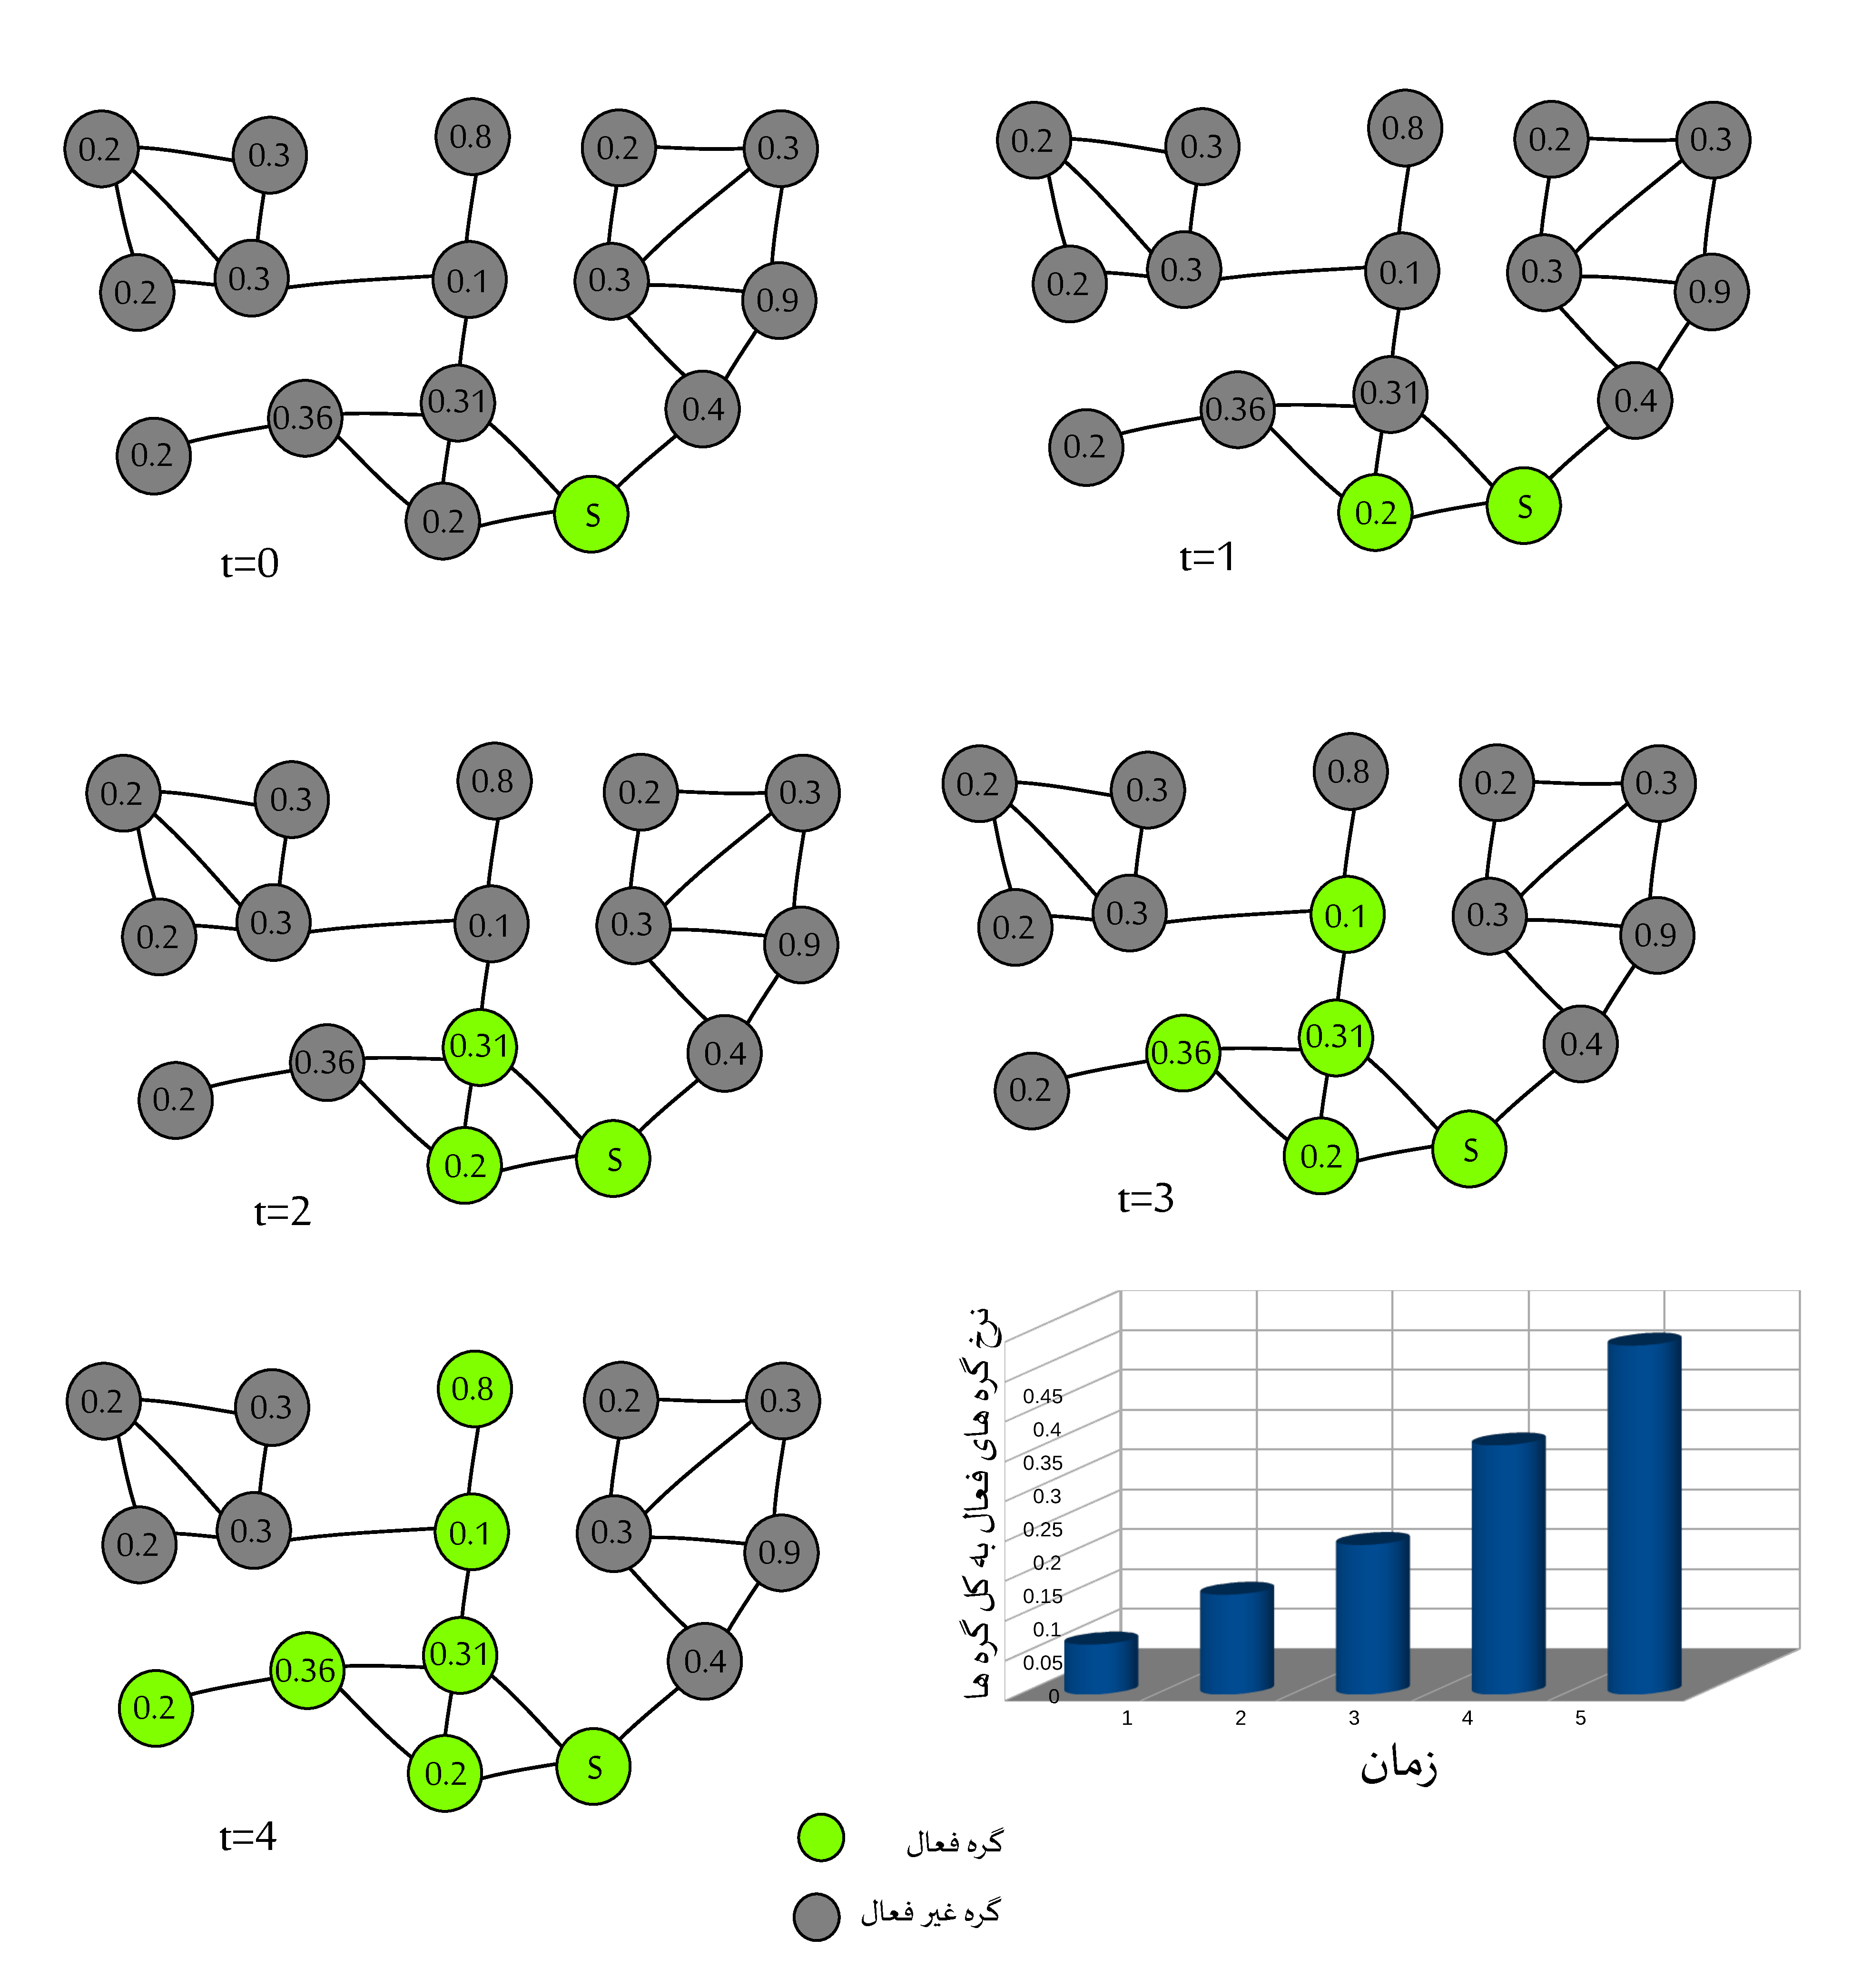
\includegraphics[scale=0.242]{figures/ltm}
 \caption[مدل آستانه خطی]
 { شبیه سازی فرایند کار مدل آستانه خطی با گره \lr{S} به عنوان گره فعال اولیه.}
\end{figure}

\subsection{مدل آستانه اکثریت}
\noindent{
 مدل آستانه اکثریت \پانویس { Majority Threshold Model} یکی از مدل‌های خانواده‌ی آستانه می‌باشد \cite{bhagat_maximizing_2012,richardson_mining_2002,rozin_negativity_2001} که به شدت مورد مطالعه قرار گرفته است. در این مدل گره $v \in V$ وقتی که آستانه $\phi_{v}={(1/2)}d(v)$ به دست بیاید فعال می‌شود \cite{wu_opportunistic_2014}. یکی از کاربرد‌های مهم این مدل در بررسی فرایند نظرسنجی‌هاست. سختی محاسباتی یافتن گره‌های اولیه‌ای که باعث حداکثر شدن گره‌های فعال شده در پایان اجرای این فرایند می‌شوند با سخطی مدل آستانه خطی برابر است.
}

\subsection{مدل آستانه کوچک}
\noindent{
 مدل آستانه کوچک \پانویس { Small Threshold Model} یکی دیگر از مدل‌های خانواده‌ی آستانه می‌باشد \cite{eiselt_competitive_1989,wu_opportunistic_2014} که در این مدل به همگی گره‌های $v \in V$ یک عدد ثابت کوچک $(\phi_v)$ به عنوان آستانه فعال سازی منتسب می‌شود. در \cite{kempe_maximizing_2003} اثبات شده است که برای $\phi_v \geqslant 3 $ مشکل یافتن گره‌های آغازین حداکثرکننده‌ی امر پخش در پایان اجرای این مدل \lr{NP-Hard} است.
}

\subsection{مدل آستانه توافق همگانی}
\noindent{
 در مدل آستانه توافق همگانی\پانویس { Unanimous Threshold Model} آستانه فعال سازی هر گره $v$ به صورت $\phi_v = d(v)$ تعیین می‌شود که $d(v)$ تعداد همسایگان گره $v$ را نشان می‌دهد. این مدل بیشترین مقاومت را نسبت به پخش تاثیر در سطح شبکه اجتماعی دارد. این مدل بیشتر برای بررسی نقاط ضعف امنیتی و بررسی امنیت شبکه‌ها به کار برده می‌شود. برای مثال یک شبکه‌ی اجتماعی را می‌توان درنظر گرفت که در حالت ایده آل یک شایعه وقتی مورد قبول فرد قرار می‌گیرد که مورد قبول همه‌ی همسایگان وی قرار گرفته باشد. یافتن بهترین مجموعه گره‌های نخستین برای بیشینه کردن انتشار در این روش نیز \lr{NP-Hard} است.
}

\subsection{دیگر انواع مدل‌های خانواده‌ی مدل‌های آستانه}
\noindent{
مدل‌های آستانه دیگر به جز موارد ذکر شده‌ی بالا را می‌توان با تعیین تابع آستانه‌ی مناسب طراحی نمود. برای نمونه می‌توان به مدل‌هایی مثل مدل آستانه‌ی خطی رنگی و مدل آستانه جدا \cite{wu_opportunistic_2014,chaintreau_impact_2007,chen_efficient_2009} و همین طور مدل آستانه‌ی متناسب با وزن اشاره نمود. ضمنا در \cite{kempe_maximizing_2003} ثابت شده است که دو مدل انتشار مستقل و آستانه‌ی خطی از نظر ریاضی معادل هم می‌باشند.
}

%\newpage
\section{مدل‌های همه‌گیری}
\noindent
{
در این بخش به معرفی و تشریح مدل‌های همه‌گیری که برای مدل‌کردن فرایند پخش اطلاعات ارایه شده اند می‌پردازیم. 
}
\subsection{مدل \texorpdfstring{\lr{SIR}}{SIR}}
\noindent{
مدل \lr{SIR}\پانویس{ \lr{ Susceptible-Infectious-Recovered}} اولین بار در \cite{m1925applications,kermack1932contributions} برای مدل‌کردن فرایند همه‌گیری بیماری‌های مسری به زبان ریاضی و تحلیلی مطرح شده است. در این مدل در ابتدا یک جمعیت ثابت اولیه به نام $\Omega$ به اندازه‌ی $N$ در نظر گرفته می‌شود. سپس سه مجموعه‌ی $S$ و $I$ و $R$ که به ترتیب نشان دهنده‌ی افراد سالم و مبتلا و افراد درمان‌یافته‌ی(و یا تلف‌شده) $\Omega$ می‌شوند را می‌سازیم. در این مدل اعضای $S$ با نرخ $\alpha$(نرخ ابتلا) به مجموعه‌ی $I$ وارد می‌شوند. هم‌چنین اعضای $I$ هم با نرخ 
$\gamma$ که زمان متوسط دوره‌ی مریضی را نشان می‌دهد، به مجموعه‌ی $R$ وارد می‌شوند. 
\\
\\
\centerline{
\scalebox{1.25}{
\begin{latin}
${\color{blue}{\mathcal{S} \xrightarrow{\alpha} \mathcal{I} \xrightarrow{\gamma } \mathcal{R}}}$
\end{latin}}}

%\\
برای اینکه بتوانیم در لحظه‌ی دلخواه $t$ مقادیر $S(t)$ و $I(t)$ و $R(t)$، که به ترتیب نشان دهنده‌ی تعداد اعضای مجموع‌های $S$ و $I$ و $R$ می‌باشند، محاسبه کنیم نیازمند حل معادله‌های زیر می‌باشیم.
\\
\begin{center}
%\scalebox{1.25}
 {
$\frac{dS}{dt} = - \alpha SI$} %+ \mu (N - S) + \gamma I
\\
%\scalebox{1.25}
 {
$\frac{dI}{dt} = \alpha SI - \gamma I$} %- \mu I 
\\
%\scalebox{1.25}
 {
$\frac{dR}{dt} = \gamma I$ %- \mu I
} 
\end{center}
%%\\
این مدل دارای چند فرض اصلی درباره‌ی روند انتشار بیمارست. برای نمونه در این مدل این فرض وجود دارد که نرخ ابتلا(شتاب پخش‌شدن) برای تمام جمعیت یکسان و برابر $\alpha$ می‌باشد. ضمنا در هر واحد زمان هرکدام از اعضای $S$ بااحتمال برابر به مجموعه‌ی $I$ می‌رود. در این مدل در آستانه‌ی بازتولید(ابتلا و شفا) به نام $\lambda$ وجود برابر 
$\lambda = {\frac{S\alpha}{\gamma}}$
می باشد. طی این رابطه وقتی در این مدل 
$\lambda < 1$ 
باشد مریضی همگیر نخواهد بود و در ابتدا انتشار آن متوقف می‌شود. و اگر 
$\lambda > 1$ 
باشد بیماری به مرور زمان همه‌ی اعضای $S$ را مبتلا خواهد نمود. و هنگامی که 
$\lambda = 1$
باشد سیستم در حال تعادل است ولی در مرز شیوع قرار دارد.

 \begin{figure}[H]
 \centering
 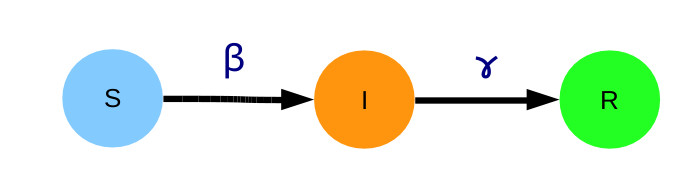
\includegraphics[scale=0.5]{figures/SIR}
 \caption[مدل \texorpdfstring{\lr{SIR}}{SIR}]
 {نمودار تعداد اعضای مجموعه‌های $S$(آبی/صاف) و $I$(سبز/خط تیره) و $R$(قرمز/خط مربع) نسبت به زمان در شبیه‌سازی مدل \lr{SIR} با جمعیت 1000.}
\end{figure}

فقط باید بدین نکته توجه داشت که در همگی مدل‌های ریاضی ارایه شده برای همه‌گیری به صورت کلی فرض بر این گذاشته شده است که $S(t) + I(t) + R(t) = N$ می‌باشد. البته در صورت حذف و یا اضافه شدن یکی از مجموعه‌های سمت چپ معادله تابع مقدار لحظه‌ای مناسب آن مجموعه هم باید حذف و یا اضافه گردد.
}


\subsection{مدل \texorpdfstring{\lr{SI}}{SI}}
\noindent{
این مدل شبیه مدل \lr{SIR} می‌باشد با این تفاوت که در این مدل فرض بر این گذاشته می‌شود که بیماری در حال همه‌گیری درمان ناپذیر است، و یا تاثیر تکنولوژی و یا خبر که در حال انتشار در جامعه می‌باشد کم ناشدنیست. برای نمونه این مدل برای توصیف فرایند شیوع بیماری ایدز و یا چگونگی روند استفاده از تلفن، اینترنت توسط مردم کاربرد دارد. 
\\
\\
\centerline{
\scalebox{1.25}{
\begin{latin}
${\color{blue}{\mathcal{S} \xrightarrow{\alpha} \mathcal{I}}}$
\end{latin}}}

معادله‌های دیفرانسیل این مدل برای محاسبه‌ی $S(t)$ و $I(t)$ در این مدل به صورت زیر خواهند بود.
\\
\begin{center}
%\scalebox{1.25}
 {
$\frac{dS}{dt} = - \alpha SI$} %+ \mu (N - S) + \gamma I
\\
%\scalebox{1.25}
 {
$\frac{dI}{dt} = \alpha SI$} %- \mu I 
\end{center}

دو معادله‌ی فوق برخلاف اکثر معادلات دیفرانسیل مربوط به خانواده‌ی مدل‌های همه‌گیری حل تحلیلی دارند، که به آن تابع رشد لوژستیک\پانویس{ \lr{ Logestic Growth Function}} می‌گویند. در زیر این تابع را که نشان‌دهنده‌ی تعداد افراد مریض جامعه می‌باشد دیده می‌شود.

% \begin{figure}[h]{0.5\textwidth}
% 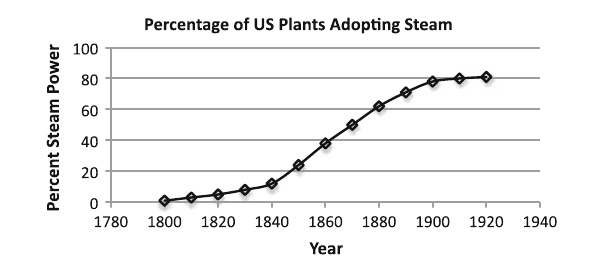
\includegraphics[width=\textwidth]{figures/SI/WaterPower}
% \caption{رشد استفاده‌ی موتور بخار در آمریکا \lr{SI}}
% \end{figure}

\begin{center}
%\scalebox{1.25}
 {
$I(t) = \frac{N I_{0}e^{\alpha t}}{N + I_{0}(e^{\alpha t} - 1)}$
\\
$I_{0}$ نشان دهنده‌ی تعداد افراد مبتلا در لحظه‌ی آغاز است. 
با فرض 
$i_{0}=\frac{I_{0}}{N}$ خواهیم داشت: \\
$i(t) = \frac{i_{0}e^{\alpha t}}{1 + Ii_{0}(e^{\alpha t} - 1)}$}
\\
\end{center}

\begin{figure}[h]
 \centering
 \begin{subfigure}[b]{0.6\textwidth}
 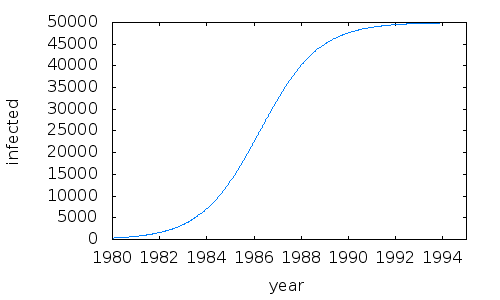
\includegraphics[width=\textwidth]{figures/SI/aids1980-95}
 \caption{رشد مبتلایان به ایدز از سال ۱۹۸۰ تا ۱۹۹۵ در آمریکا.}
 \end{subfigure}%
 
 %add desired spacing between images, e. g. ~, \quad, \qquad, \hfill etc.
 %(or a blank line to force the subfigure onto a new line)
 \begin{subfigure}[b]{0.6\textwidth}
 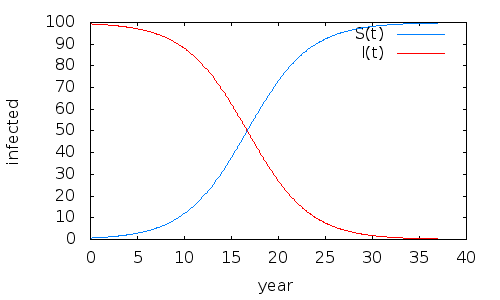
\includegraphics[width=\textwidth]{figures/SI/aidsSt-It}
 \caption{شبیه سازی مدل \lr{SI}}
 \end{subfigure}
 
 \caption[شبیه‌سازی مدل \texorpdfstring{\lr{SI}}{SI}]
 {شبیه‌سازی همه‌گیری به کمک مدل \lr{SI} با تابع رشد لوژستیک 
 $\frac{50000}{1+e^{5+(-0.8)x}}$.}
\end{figure}
}

\subsection{مدل \texorpdfstring{\lr{SIS}}{SIS}}
\noindent{
این مدل بسیار شبیه مدل \lr{SIR} می‌باشد با این تفاوت که در این مدل فرض بر این گذاشته می‌شود که بیماران(اعضای $I$) بعد از گذراندن بیماری شفا می‌یابند و به مجموعه‌ی $S$ بر‌می‌گردند. به زبان ساده در این مدل پس از ابتلا بعد از مدتی عضو بیمار دوباره به اجتماع افراد سالم مستعد بیماری باز می‌گردد.
\\
\\
\centerline{
\scalebox{1.25}{
\begin{latin}
${\color{blue}{\mathcal{S} \xrightarrow{\alpha} \mathcal{I} \xrightarrow{\gamma } \mathcal{S}}}$
\end{latin}}}

معادله‌های دیفرانسیل این مدل برای محاسبه‌ی $S(t)$ و $I(t)$ به صورت زیر خواهند بود.
\\
\begin{center}
%\scalebox{1.25}
 {
$\frac{dS}{dt} = - \alpha SI + \gamma I$} %+ \mu (N - S) + \gamma I
\\
%\scalebox{1.25}
 {
$\frac{dI}{dt} = \alpha SI - \gamma I$} %- \mu I 
\end{center}

}

یک تفاوت عمده‌ی این مدل با مدل \lr{SIR} و \lr{SI} در امکان از بین نرفتن بیماری و یا عامل‌ همه‌گیر در یک جامعه‌ می‌باشد. به زبان ساده‌تر چرخه ابتلا و شفا می‌تواند تا ابد در جامعه تکرار شود.

\subsection{مدل \texorpdfstring{\lr{SIRS}}{SIRS}}
\noindent{
این مدل هم بسیار شبیه مدل $SIR$ می‌باشد با این تفاوت که اعضای مجموعه‌ی $R$ بعد از مدتی به مجموعه‌ی $S$ می‌پیوندند.
\\
\\
\centerline{
\scalebox{1.25}{
\begin{latin}
${\color{blue}{\mathcal{S} \xrightarrow{\alpha} \mathcal{I} \xrightarrow{\gamma } \mathcal{R}} \xrightarrow{\frac{1}{\sigma}} \mathcal{S}}$
\end{latin}}}

معادله‌های دیفرانسیل این مدل برای محاسبه‌ی مقادیر $S(t)$ و $I(t)$ و $R(t)$، به صورت زیر خواهند بود.

\begin{center}
%\scalebox{1.25}
 {
$\frac{dS}{dt} = - \alpha SI + \sigma R$}
\\
%\scalebox{1.25}
 {
$\frac{dI}{dt} = \alpha SI - \gamma I$} 
\\
%\scalebox{1.25}
 {
$\frac{dR}{dt} = \gamma I - \sigma R$}

\end{center}

}

\subsection{دیگر مدل‌های همه‌گیری}
\noindent{
مشتقات زیادی از مدل \lr{SIR} برای مدل‌سازی فرایند همه‌گیری و پخش بیماری و همین‌طور انتشار شایعه در سطح جوامع انسانی مطرح شده است. برای مثال به‌جز مدل‌های همه‌گیری ذکر‌شده تا به الآن در این نوشته، مدل‌های \lr{SEIS} و \lr{SEIR} و \lr{MSIR} و \lr{MSEIR} و \lr{MSEIRS} و \lr{SEIZ} \cite{hethcote2000mathematics} که همگی جزو مدل‌های احتمالی همه‌گیری می‌باشند، نیز برای مدل‌سازی پخش اطلاعات به ‌کار رفته اند. در مدل‌های فوق الذکر حرف \lr{M}\پانویس{ \lr{Maternally-derived immunity}} نشاندهنده‌ی حالتی است که فرد در ابتدا برای مدتی دارای مصونیت به عامل همه‌گیری است. حروف \lr{E}\پانویس{ \lr{Exposed}} و \lr{Z}\پانویس{ \lr{Maternally-derived immunity}} هم به ترتیب معنای حالت‌های نهفتگی بیماری و حالت شک به صحت اطلاعات از جانب فرد مطلع(این مدل درباره‌ی مدل‌سازی شایعه کاربرد دارد) می‌باشند. 
}

\begin{figure}[h]
 \centering
 \begin{subfigure}[b]{0.32\textwidth}
 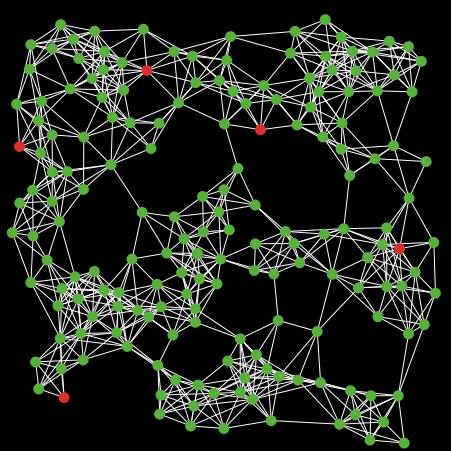
\includegraphics[width=\textwidth]{figures/SIRS/t0}
 \caption{وضعیت جامعه در $t=0$}
 
 \end{subfigure}%
 ~ %add desired spacing between images, e. g. ~, \quad, \qquad, \hfill etc.
 %(or a blank line to force the subfigure onto a new line)
 \begin{subfigure}[b]{0.32\textwidth}
 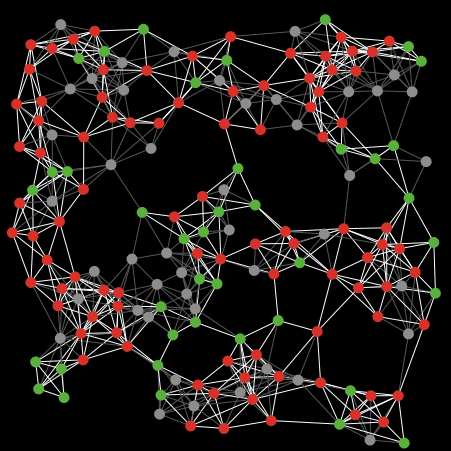
\includegraphics[width=\textwidth]{figures/SIRS/t223}
 \caption{وضعیت جامعه در $t=223$}
 
 \end{subfigure}
 ~ %add desired spacing between images, e. g. ~, \quad, \qquad, \hfill etc.
 %(or a blank line to force the subfigure onto a new line)
 \begin{subfigure}[b]{0.32\textwidth}
 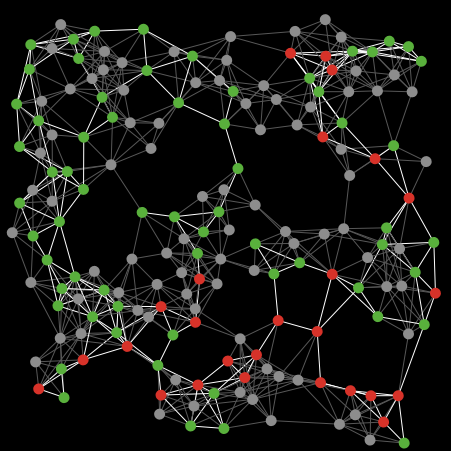
\includegraphics[width=\textwidth]{figures/SIRS/t540}
 \caption{وضعیت جامعه در $t=540$}
 %\label{fig:mouse}
 \end{subfigure}
 ~ %add desired spacing between images, e. g. ~, \quad, \qquad, \hfill etc.
 %(or a blank line to force the subfigure onto a new line)
 
 
 \begin{subfigure}[b]{0.4\textwidth}
 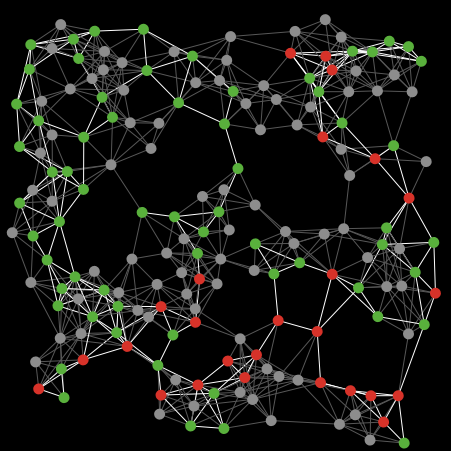
\includegraphics[width=\textwidth]{figures/SIRS/t540}
 \caption{وضعیت جامعه در پایان شبیه‌سازی}
 
 \end{subfigure}
 ~~~
 \begin{subfigure}[b]{0.35\textwidth}
 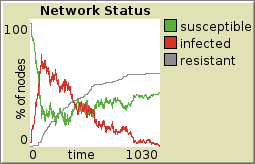
\includegraphics[width=\textwidth]{figures/SIRS/SIRS}
 \caption{نمودار وضعیت جامعه در طی شبیه‌سازی}
 
 \end{subfigure}
 \caption[شبیه‌سازی مدل \texorpdfstring{\lr{SIRS}}{SIRS}]{شبیه‌سازی همه‌گیری به کمک مدل \lr{SIRS} با $\alpha=0.025$ و ${\frac{1}{\sigma}} ={\gamma}=0.05.$ و $N=175$.
 (رنگ قرمز و سبز و خاکستری به ترتیب افراد بیمار و سالم و افراد شفا ‌یافته‌ی جامعه را نشان می‌دهند.)}
\end{figure}

\section{مدل‌های دیگر پخش اطلاعات}
\noindent{
جدا از سه دسته مدل مطرح که گفته شد مدل‌های دیگری هم برای مدل‌کردن فرایند پخش اطلاعات ارایه شده اند
\cite{kwon_information_2009,hajibagheri_modeling_2013,broecheler_scalable_2010,kim_modeling_2011,sotoodeh_general_2013,he_influence_2012,jiang_modeling_2014,snijders_introduction_2010,hurd_watts_2013,wang_modeling_2013,lande_model_2008,lou_social_2014,lou_modeling_2014,cheng_epidemic_2013}.
اکثر این مدل‌ها از مدل‌های گفته شده قبلی مشتق شده اند. البته مدل‌های دیگری نیز برای امر پخش در سطح شبکه‌های پیچیده ارایه شده اند، مانند \cite{lin_modelling_2014} که مسئله‌ی پخش با چند منبع را به صورت خاص مورد مطالعه قرار داده اند. 

}

 \begin{figure}[H]
 \centering
 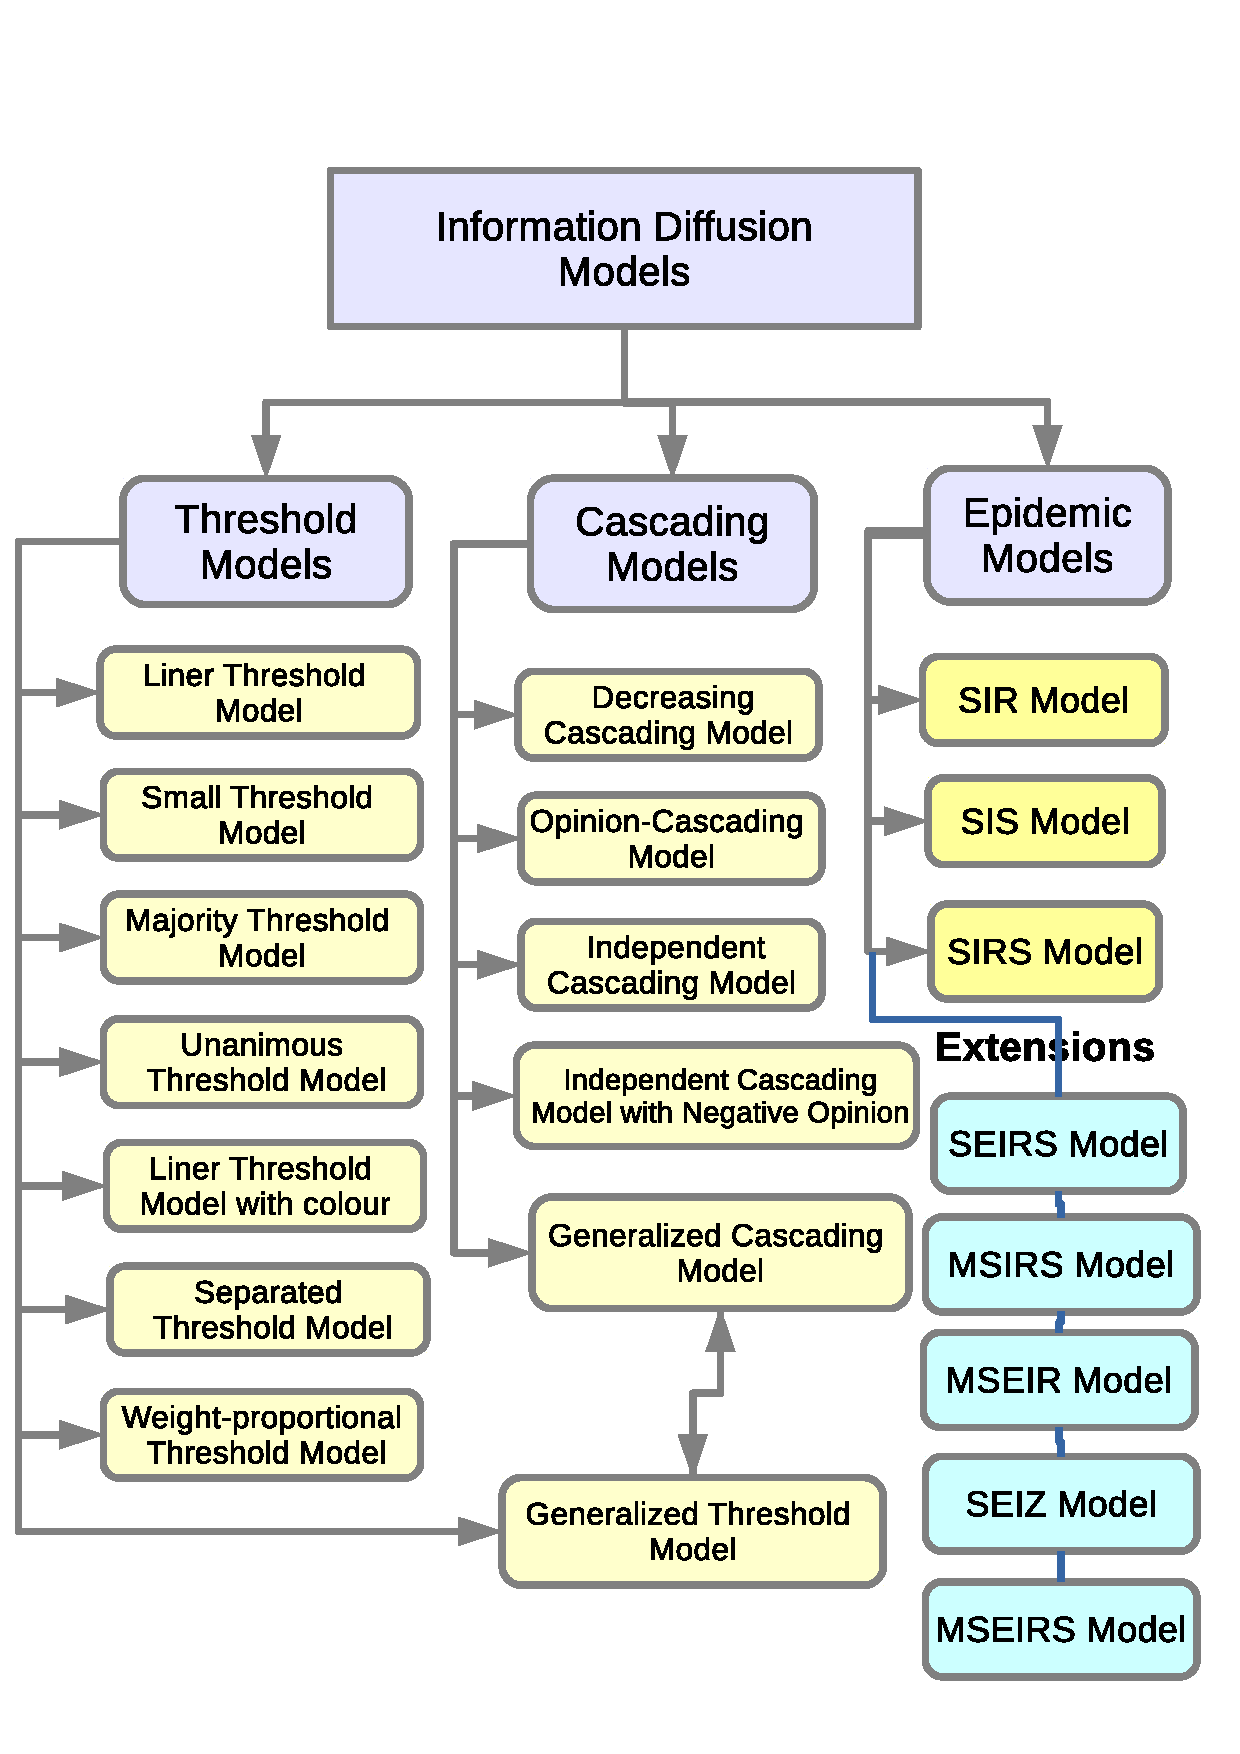
\includegraphics[scale=0.6]{figures/IDMO}
 \caption[مدل‌های اصلی پخش اطلاعات]
 {نمایی کلی از خانواده مدل‌های اصلی پخش اطلاعات.}
\end{figure}

\section{خلاصه‌ی مطالب فصل}
\noindent{
در این فصل سه گروه اصلی از مدل‌های پخش اطلاعات معرفی شدند. سه خانواده‌ی معرفی شده شامل مدل‌های آستانه و انتشار و همه‌گیری بیماری می‌باشند. مدل‌های \lr{LT} و \lr{IC} بسیار محبوب محققان برای مد‌سازی فرایند پخش اطلاعات می‌باشند و در ابتدا برای یافتن روشی الگوریتمیک برای به حداکثر رساندن تاثیر اجتماعی مطرح شدند. یافتن $k$ گره‌ای که فرایند پخش را حداکثر کنند در این مدل از نظر محاسباتی جزو دسته مسائل \lr{NP-Hard} می‌باشد، لذا الگوریتم‌های هیوریستیک زیادی برای این دو مدل مانند الگوریتم‌های \lr{CELF} و \lr{CELF++} و \lr{SIMPATH} \cite{kempe_maximizing_2003,chen_scalable_2010,lv_improved_2014,goyal_simpath:_2011} تا به امروز ارایه شده اند.
\\
\indent
مدل‌های همه‌گیری مطرح و مورد استفاده هم مانند \lr{SIR} و \lr{SIRS} و \lr{SIS} در این فصل توضیح داده شدند. پخش اطلاعات دارای شباهت‌های زیادی با فرایند همه‌گیری بیماری‌ دارد، به طوری که مدل‌های همه‌گیری فوق الذکر در اکثر موارد توانسته اند برآورد درستی نسبت به روند واقعی فرایند پخش 
اطلاعات به دست بدهند.

}
\end{persian}

\chapter{نتیجه گیری} 

\newpage

\section{جمع بندی}
\noindent{
شبکه‌های اجتماعی خصوصیات منحصر به فردی دارند که آن‌ها را از دیگر شبکه‌ها متمایز می‌سازد. این خوصیات در بسیاری از لحاظ برای تولید مدل‌های پخش اطلاعات ساده سازی شده اند. به طور کلی از میان روش های زیادی که برای مدل‌کردن فرایند پخش اطلاعات در شبکه‌های اجتماعی مطرح شده اند دو مدل \lr{LT} و \lr{IC} مورد استقبال زیادی قرار گرفته اند. در این دو مدل که برای بار اول در سال ۲۰۰۳ برای ارایه مدلی برای حداکثر نمودن تاثیر اجتماعی میان اعضای یک شبکه‌ی اجتماعی ارایه گردیده اند، برای یافتن $k$ فردی که در پایان شبیه سازی تاثیر را به حداکثر برسانند الگوریتم‌های هیوریستیک زیادی مطرح شده اند که در حدود 63 درصد را پوشش می دهند. لذا اکثر این الگوریتم‌ها از مشکل مقیاس‌ناپذیری\پانویس{ \lr{Non-Scalablility}} در بعد اندازه‌ گراف مورد مطالعه رنج می برند. \\
در کنار این دو مدل‌های ریاضی همه‌گیری بیماری که معروف ترینشان مدل‌های \lr{SIR} و \lr{SIRS} و \lr{SIS} و \lr{SI} می‌باشند در چند سال اخیر برای مدل‌کردن فرایند پخش اطلاعات از مدل کردن پخش شایعه تا مدل کردن انتشار رفتار و خبر استفاده شده اند. این محققان در این مدل‌ها و مشتقات آن‌ها تغییراتی وارد نموده اند تا در بستر گراف یک شبکه‌ی اجتماعی قابل استفاده باشند. 
 
}
\section{کار های آتی}
\noindent{
اکثر مدل‌های پخش اطلاعات که در این گزارش ذکر شدند به صورت موضعی و بر روی مجموعه‌های مشخصی از داده‌های شبکه‌هایی هم چون توییتر و فیسبوک و چند شبکه اجتماعی معروف دیگر ازمایش گردیده اند. لذا تعمیم این که رفتار کاربران همه‌ی شبکه‌های اجتماعی موجود در اینترنت با وجود امکانت متنوع و گستردگی زیاد سرویس‌های آن‌ها در فرایند پخش اطلاعات به یک گونه باشد کار بیهوده‌ای است. از طرفی خیلی از این مدل‌ها یک تصویر لحظه‌ای از شبکه اجتماعی را مورد مطالعه قرار می‌دهند، ضمنا این مدل‌ها بسیاری از خصوصیات اصلی یک شبکه اجتماعی مثل هوموفیلی میان کاربران و قدرت اتصال‌های میان افراد را در کار خود تاثیرگذار نمی‌کنند. برای همین این مدل‌ها خوصیات منحصر به فرد شبکه ‌های اجتماعی که‌ آن‌ها را از مابقی شبکه‌های ارتباطی و شبکه‌های دنیای واقعی متمایز می‌سازند در مدل خود به خوبی لحاظ ننموده اند.
\\
از طرفی بحث این‌که آیا امکان پیش‌بینی امر انتشار چیزی مانند شایعه در یک شبکه‌ی اجتماعی وجود دارد موردیست که در چند سال اخیر بسیار مورد توجه قرارگرفته است ولی کار انجام شده از لحاظ طراحی مدل‌های بهتر و دقیق تر با فرض قابل پیش‌بینی بودن امر انتشار امکان بهبود را دارد. ضمنا موضوعاتی مانند یافتن افراد تاثیر گذار در امر پخش اطلاعات، همین طور ارایه مدل‌هایی که پویایی گراف شبکه‌ی اجتماعی را به خوبی دربر بگیرند نیز می‌توانند از موضوعات جذاب برای پژوهش در این زمینه باشند.
}



\begingroup
\inputencoding{latin1}
\settextfont[Scale=1.25]{Times New Roman}
\renewcommand{\baselinestretch}{1.1} 
\pagestyle{empty}
{
\bibliographystyle{ieeetr-fa}%{chicago-fa}%{acm-fa}%{plainnat-fa}%{unsrt-fa}%{asa-fa}%{plain-fa}
\bibliography{bibs/main,bibs/add,bibs/dummy_refs}

}
%\nocite{*}
\endgroup

\chapter*{واژه‌نامه فارسی به انگلیسی}\markboth{واژه‌نامه فارسی به انگلیسی}{واژه‌نامه فارسی به انگلیسی}
\addcontentsline{toc}{chapter}{واژه‌نامه فارسی به انگلیسی}
\thispagestyle{empty}

\englishgloss{Probabilistic}{احتمالی}
\englishgloss{Information Diffusion}{پخش اطلاعات}
\englishgloss{Process}{فرایند }
\englishgloss{Mark Granovetter}{مارک گرانووتر}
\englishgloss{Meme}{میم}
\englishgloss{Graph}{گراف}
\englishgloss{Threshold Model}{مدل آستانه}
\englishgloss{Majority}{اکثریت}
\englishgloss{Reducing}{کاهشی}
\englishgloss{Topic}{عنوان}
\englishgloss{Message}{پیام}
\englishgloss{Bursty Topic}{عنوان آنی}
\englishgloss{User}{کاربر}
\englishgloss{Rumour}{شایعه}
\englishgloss{Diffusion of Innovation}{پخش نوآوری}
\englishgloss{HashTag}{هشتگ}
\chapter*{واژه‌نامه  انگلیسی به  فارسی}\markboth{واژه‌نامه  انگلیسی به  فارسی}{واژه‌نامه  انگلیسی به  فارسی}
\addcontentsline{toc}{chapter}{واژه‌نامه  انگلیسی به  فارسی}
\thispagestyle{empty}

\persiangloss{انتشار}{Cascade}
\persiangloss{شبکه پیچیده}{Complex Network}
\persiangloss{اندازه }{Measure}
\persiangloss{همه‌گیری}{Pandemic}
\persiangloss{مدل سرایت}{Epidemic Model}
\persiangloss{احتمالی}{Probabilistic}
\persiangloss{اتصال}{Link}
\persiangloss{یال}{Edge}
\persiangloss{گره}{Node}
\persiangloss{راس}{Vertex}
\persiangloss{قانون توانی}{Powr Law}
\persiangloss{شبکه اجتماعی}{Social Network}
\persiangloss{اجتماع}{Community}
\persiangloss{خوشه}{Cluster}
\persiangloss{ان-پی تمام}{NP-Complete}
\persiangloss{پدیده‌ی جهان کوچک}{Small World Phenomenon}
\persiangloss{مستعد بیماری}{Susceptible}
\persiangloss{پخش کننده‌ی بیمار}{Infectious}
\persiangloss{از چرخه ‌‌بیماری ‌خارج ‌شده}{Removed}
\persiangloss{موافق}{Unanimous}


\end{document}



